\documentclass[preprint,12pt]{elsarticle}

\usepackage{amsmath,amssymb,amsthm,bm}
\usepackage{booktabs}
\usepackage{enumitem}
\usepackage{graphicx}
\usepackage{microtype}
\usepackage{xcolor}
\usepackage{hyperref}
\hypersetup{hidelinks,hypertexnames=false}
\usepackage{placeins}
\usepackage{url}
\usepackage{float}
\usepackage{array}
\setlength{\emergencystretch}{2em}

\journal{Future Internet}

\newtheorem{proposition}{Proposition}
\newtheorem{remark}{Remark}
\newcommand{\E}{\mathbb{E}}
\newcommand{\Prob}{\mathbb{P}}
\newcommand{\Aset}{\mathcal{A}}
\newcommand{\Cset}{\mathcal{C}}

\begin{document}

\begin{frontmatter}

\title{Guarded Multi-Fidelity Optimization with Trace-Derived Risk Auditing for Privacy-Constrained Cloud--Edge LLM Serving}

\author[utabuk]{Abdulaziz M. D. Aljohani\corref{cor1}}
\ead{a-aljohani@ut.edu.sa}
\author[utabuk]{Khaled M. Alhawiti}
\ead{khalhawiti@ut.edu.sa}

\cortext[cor1]{Corresponding author.}
\affiliation[utabuk]{organization={Faculty of Computers and Information Technology, University of Tabuk},
  city={Tabuk}, postcode={47512}, country={Saudi Arabia}}

\begin{abstract}
Privacy-constrained cloud--edge LLM services must activate remote capacity before local pressure causes admission loss while avoiding unnecessary cloud cost. We study 190 two-threshold policies using a compound-jump simulator and a reflected-diffusion screen. Diffusion-Residual Bayesian Guarded Search (DR-BGS) combines affine calibration, Gaussian-process residual learning, and structural anchors. On 36 exhaustively evaluated synthetic scenarios, a 20-policy budget reduces high-fidelity replications by 88.77\%; all 180 selections remain within 1\% of exhaustive training selection on independent holdout streams, with 0.348\% maximum excess. A chronologically split BurstGPT study then separates nomination from certification. Under 2\% protected-request and 5\% eligible-request blocking limits, all 120 method runs abstain, and exhaustive auditing finds 0 of 2,280 certifiable policy--scenario pairs at the original load ratios. Increasing certification evidence does not rescue those regimes. An exploratory frontier identifies load reduction as the most consistent route to feasibility. A separately locked seven-day robustness replication uses 11,810 search and 6,086 later certification records: it again finds 0 of 2,280 high-load certifiable pairs, while all 18 cross-method-distinct low-load scenario--policy pairs pass two disjoint 1,200-replay batches. The results distinguish efficient nomination, operational feasibility, and independent certification, without claiming production safety.
\end{abstract}

\begin{keyword}
cloud--edge computing \sep LLM serving \sep simulation optimization \sep multi-fidelity modeling \sep risk certification \sep trace replay \sep privacy-constrained routing
\end{keyword}

\end{frontmatter}

\section{Introduction}
\label{sec:intro}

Hybrid cloud--edge inference offers a clear privacy boundary: sensitive requests remain on premises, while eligible traffic may use remote capacity. The operating problem is less simple. Local throughput changes with active-sequence count, batching, and KV-cache pressure \cite{kwon2023pagedattention,patel2024splitwise,zhong2024distserve,agrawal2024sarathi}. Remote capacity can require model loading, container startup, or session establishment before accepting work \cite{serverlessllm2024}. Late activation causes local admission loss; early activation pays for capacity that may not be needed.

We represent the controller by a hysteretic pair
\[
0<\alpha_{\rm off}\le \alpha_{\rm on}<K,
\]
where cloud preparation starts at $\alpha_{\rm on}$ and release is allowed only below $\alpha_{\rm off}$. A 19-level triangular grid contains 190 policies. Exhaustive high-fidelity evaluation is therefore expensive even before independent validation.

The paper uses two stochastic fidelities. The reference is a compound-jump event simulator with delayed cloud activation, whole-request admission, finite local pressure capacity, and privacy classes. A stationary reflected diffusion supplies the full policy surface cheaply, but its absolute blocking and delay metrics are not accurate enough to support operational claims. Diffusion-Residual Bayesian Guarded Search (DR-BGS) uses that approximation only as a mechanistic trend, learns the residual with a Gaussian process, and reserves high-fidelity evaluations for 20 structurally selected policies. Boundary and diagonal anchors protect regions where the diffusion ranking can fail.

The original synthetic benchmark establishes simulation efficiency, but synthetic success alone does not answer two questions important to a cloud--edge system: does the search survive trace-derived burst structure, and can a selected policy be accepted only when independent evidence supports a declared risk statement? To address both, we add a chronologically split BurstGPT-derived study and an explicit certification gate. The original locked study uses the first 100 chronological rows of the official \texttt{BurstGPT\_1.csv} release; a separately locked robustness replication expands the workload basis to a fixed seven-day window. Arrival times and token counts are trace-derived, while privacy labels remain synthetic because the public workload does not identify request sensitivity. Moving-block resampling preserves short local ordering, and search and certification use disjoint chronological pools and disjoint simulation seeds.

The study intentionally distinguishes nomination from certification. DR-BGS nominates a policy under a fixed simulation budget. Independent high-fidelity replications then form Bernoulli violation indicators. Simultaneous one-sided Clopper--Pearson upper bounds decide whether a claim is certified; otherwise the procedure abstains. This is post-selection simulation certification, not SafeOpt-style safe exploration \cite{sui2015safeopt}, and it does not make the low-fidelity model a safety model.

The paper makes five contributions.
\begin{enumerate}[leftmargin=*]
\item \textbf{A cloud--edge service model.} A delayed hybrid LLM controller combines privacy-restricted routing, finite local workload pressure, compound request jumps, and two-threshold cloud activation.
\item \textbf{A guarded multi-fidelity search.} DR-BGS combines a mechanistic diffusion trend, residual GP learning, and structural anchors for a finite triangular hysteresis policy space.
\item \textbf{Controlled optimizer evidence.} Equal-budget comparisons, component ablations, exhaustive 190-policy surfaces, and a direct ranking-and-selection comparator separate the effect of structural guards from the diffusion residual.
\item \textbf{Chronologically separated trace-derived evaluation.} A compact public BurstGPT slice supplies arrival and token structure for search and later certification pools. The exact slice, transformation, hashes, and replay code are archived.
\item \textbf{Evidence gating and operating-envelope diagnosis.} Exact simultaneous risk bounds are applied after selection. The locked high-load study retains universal abstention; exhaustive auditing determines whether the policy family contains any certifiable alternative; an exploratory frontier separates operational infeasibility from evidence limitation; and a separately locked low-load confirmation shows that the unchanged gate can return stable positive decisions in an interior feasible regime.
\end{enumerate}

The strongest result is not that every selected policy is safe. At the original load ratios, exhaustive auditing finds no certifiable policy and the gate abstains. At a separately locked low-load point, the same gate certifies every unique nominated policy in two disjoint batches. The combined evidence therefore separates search accuracy, operational feasibility, and statistical support rather than converting optimizer performance into a safety claim.
\section{Related work and novelty boundary}
\label{sec:related}

\subsection{LLM serving and cloud--edge routing}

PagedAttention, Splitwise, DistServe, and Sarathi-Serve address memory management and throughput--latency tradeoffs inside LLM-serving systems \cite{kwon2023pagedattention,patel2024splitwise,zhong2024distserve,agrawal2024sarathi}. AlpaServe, SHEPHERD, Llumnix, InfiniGen, CachedAttention, Mooncake, and provider-scale KV-cache studies add multiplexing, migration, cache movement, reuse, and deployment characterization \cite{alpaserve2023,shepherd2023,llumnix2024,infinigen2024,cachedattention2024,mooncake2025,kvcachewild2025}. These systems motivate state-dependent service and finite local capacity; they do not solve the finite simulation-allocation problem studied here.

FrugalGPT and RouteLLM select models or endpoints according to predicted quality and cost \cite{frugalgpt2024,routellm2025}. Privacy-aware cloud--edge collaboration, QoS-aware edge-expert routing, and cloud--edge--device routing thresholds have also been studied \cite{prism2026,qosrouting2025,consroute2026}. Here privacy classification precedes routing, high-sensitivity traffic is excluded from the cloud action set, and the decision variables are delayed activation and release thresholds. No cryptographic or classifier-accuracy claim is made.

BurstGPT records real temporal and token-length variation in LLM workloads \cite{burstgpt2025}. The original locked trace experiment uses the first 100 chronological rows of the official \texttt{BurstGPT\_1.csv} release, verified row-for-row against the archived source file; 95 rows have positive token counts. A separately locked robustness replication uses the first seven trace days, containing 17,896 positive-token rows. Neither study claims full-corpus representativeness. Their purpose is reproducible chronological-shift testing rather than statistical characterization of the complete BurstGPT release.

\subsection{Simulation optimization and multi-fidelity search}

Simulation optimization covers expensive stochastic evaluations, metamodels, finite alternatives, and ranking-and-selection procedures \cite{amaran2016review}. Classical procedures combine subset selection, indifference zones, common random numbers, and computing-budget allocation \cite{boesel2003cleanup,chick2001crn,chen2008subset}. Gaussian-process Bayesian optimization and discrepancy models provide established tools for expensive black-box and multi-information-source optimization \cite{jones1998ego,snoek2012bo,kennedy2000multifidelity,poloczek2017mis,kandasamy2017mfbo}. Robust and input-dependent multi-fidelity methods address unreliable or spatially variable low-fidelity information \cite{mikkola2023rmfbo,fan2024imfbo}. DR-BGS does not replace those general frameworks. It specializes a familiar affine-trend-plus-GP construction to a mechanistic compound-jump/diffusion pair and adds fixed guards for an ordered triangular policy space.

\subsection{Safe and constrained optimization versus post-selection certification}

Safe and constrained Bayesian optimization controls the points sampled during optimization or models expensive feasibility constraints \cite{gardner2014constrained,sui2015safeopt,lubsen2024safemultitask}. Our procedure has a different scope. Search may evaluate policies that would not be deployed. After a policy is nominated, independent simulator replications test a prespecified operational claim. Exact binomial bounds and a multiplicity correction determine whether the evidence is sufficient. This design cannot guarantee safety during search, nor can it transfer simulation validity to a real system. Its advantage is narrower: the final decision statement is separated from the GP model and can return ``abstain.''

\subsection{Stochastic model foundation}

Markov-modulated fluid and Poisson models provide classical representations of bursty workloads \cite{anick1982stochastic,fischer1993mmpp}. Reflected and switching diffusions have established invariant-measure theory \cite{jang2008reflected,yin2010hybrid,shao2018invariant,kang2014stationary}; constrained-diffusion invariant measures can be approximated numerically \cite{budhiraja2014numerical}. These results justify a reflected switching diffusion as a screening model. No new general theorem for reflected diffusions is claimed.
\section{System and two-threshold policy}
\label{sec:model}

\subsection{Workload classes and pressure state}

Requests belong to a high-privacy class $H$ or a cloud-eligible class $L$. Nominal arrivals are independent Poisson processes with rates $\nu_H$ and $\nu_L$; bursty Markov-modulated arrivals are used as an out-of-model stress test. A locally admitted class-$k$ request adds a random workload-pressure jump $J_k$ with distribution $F_k$, mean $m_k$, and second moment $m_k^{(2)}$.

The state
\[
X(t)\in[0,K]
\]
is a normalized local workload-pressure index. It is not a physical count of KV-cache blocks. The service law is
\[
s_n(x)=s_{0,n}\exp(-\beta_n x/K),
\]
interpreted as effective pressure relief. The empirical calibration in Section~\ref{sec:calibration} supports the law's shape and parameter range rather than a universal hardware constant.

\subsection{Cloud phase and hysteresis}

Let $N(t)\in\{0,1,2\}$ denote cloud inactive, activation in progress, and cloud active. The policy is
\[
a=(\alpha_{\rm on},\alpha_{\rm off})\in\Aset,
\qquad
0<\alpha_{\rm off}\le\alpha_{\rm on}<K.
\]
The low-fidelity phase generator is
\[
T_a(x)=
\begin{pmatrix}
-\gamma_a(x)&\gamma_a(x)&0\\
0&-\theta&\theta\\
\mu_a(x)&0&-\mu_a(x)
\end{pmatrix},
\]
with
\[
\gamma_a(x)=\nu_L\mathbf 1_{\{x\ge\alpha_{\rm on}\}},
\qquad
\mu_a(x)=\bar\mu_c\mathbf 1_{\{x<\alpha_{\rm off}\}}.
\]
Thus the nominal threshold rule starts cloud preparation when an eligible arrival observes $x\ge\alpha_{\rm on}$; completion occurs after an exponential delay with mean $1/\theta$. Cloud mode is released only after pressure falls below the lower threshold and the deactivation timer completes. The high-fidelity simulator also contains a fixed safety trigger: if an eligible request would overflow local capacity while the cloud is inactive, that request is rejected and activation starts even when $x<\alpha_{\rm on}$. The rejected request is not offloaded. This overflow trigger is deliberately absent from $T_a$ and is one source of low--high-fidelity discrepancy.

\subsection{Compound-jump reference process}

Between events, local pressure follows the deterministic service flow; arrivals create compound jumps:
\[
dX(t)=-s_{N(t)}(X(t))\,dt
+\sum_{k\in\mathcal K_{N(t)}}J_k\,dA_k(t),
\]
where $\mathcal K_0=\mathcal K_1=\{H,L\}$ and $\mathcal K_2=\{H\}$. The reference simulator contains no additional Brownian forcing. It applies whole-request admission: an $H$ arrival is blocked when $X^-+J_H>K$, and an $L$ arrival is offloaded only in phase 2. Before activation, an overflowing $L$ request is rejected rather than served immediately by the cloud. The service flow is reflected at zero; positive jumps that exceed $K$ are rejected rather than reflected.

\section{Stationary low-fidelity model}
\label{sec:diffusion}

Using the standard second-order Kramers--Moyal truncation \cite{gardiner2009stochastic}, the diffusion approximation has phase-dependent drift and variance
\[
b_n(x)=-s_n(x)+\sum_{k\in\mathcal K_n}\nu_km_k,
\qquad
a_n(x)=\sum_{k\in\mathcal K_n}\nu_km_k^{(2)}.
\]
The variance comes entirely from the arrival jumps; no exogenous diffusion term is present in the reference simulator.
The reflected process is
\[
dX(t)=b_{N(t)}(X(t))\,dt+\sqrt{a_{N(t)}(X(t))}\,dB(t)
+dL_0(t)-dL_K(t).
\]
For fixed $a$, the stationary density vector $\boldsymbol\pi^a$ satisfies
\[
\frac12\frac{d^2}{dx^2}[\boldsymbol\pi^a(x)A(x)]
-\frac{d}{dx}[\boldsymbol\pi^a(x)B(x)]
+\boldsymbol\pi^a(x)T_a(x)=0
\]
on the intervals separated by $\alpha_{\rm off}$ and $\alpha_{\rm on}$, with zero boundary flux, transmission conditions, and unit mass.

The implementation uses a nearest-neighbour continuous-time Markov-chain discretization and a generic sparse stationary solve. No specialized linear-time complexity claim is made.

Let $p^a(x)=\sum_n\pi_n^a(x)$. The main quantities are
\[
W_D(a)=\frac{\int_0^K xp^a(x)\,dx}{\Lambda_{\rm adm,D}(a)},
\]
\[
B_{H,D}(a)=\int_0^K\overline F_H(K-x)p^a(x)\,dx,
\]
and the analogous low-privacy loss $B_{L,D}(a)$ before activation. For the nominal Poisson inputs, the arrival-seen interpretation follows PASTA \cite{wolff1982pasta}. In the jump simulator, $R_{C,J}$ is offloaded class-$L$ workload divided by offered class-$L$ workload. The diffusion uses phase-2 occupancy, $R_{C,D}=\Prob_D\{N=2\}$, as its Poisson/PASTA proxy. Their difference under bursty arrivals is part of the modeled fidelity discrepancy. The objective is
\[
J_M(a)=c_WW_M(a)+c_BB_{H,M}(a)+c_LB_{L,M}(a)+c_CR_{C,M}(a),
\qquad M\in\{D,J\}.
\]
The weights are scenario inputs, not universal constants.

For the continuous-state characterization below, fix a policy
$a=(\alpha_{\rm on},\alpha_{\rm off})$. Assume: (A1) the reflected
switching diffusion has a well-posed Feller martingale problem on the compact
state space $[0,K]\times\{0,1,2\}$; (A2) $a_n$ is continuous and uniformly
elliptic, and $b_n$ is bounded and piecewise Lipschitz on the intervals
separated by $\alpha_{\rm off}$ and $\alpha_{\rm on}$; (A3) the switching
intensities are bounded and piecewise continuous, have finite one-sided limits
at both policy interfaces, and define a communicating phase graph over the
accessible state space; (A4) the joint process is topologically irreducible;
and (A5) normal reflection is imposed at $0$ and $K$. These are modeling
assumptions, not consequences of the empirical service-law fit.

\begin{proposition}[Literature-backed fixed-policy stationary characterization]
\label{prop:invariant}
Under (A1)--(A5), the fixed-policy reflected switching diffusion admits a
unique invariant probability measure. On each open interval separated by the
two thresholds, its phase components have interior densities satisfying the
stationary adjoint equations, with zero probability current at $0$ and $K$ and
weak transmission balance at both policy interfaces.
\end{proposition}

\paragraph{Justification}
This proposition records the stationary equations used by the screening model;
it is not a new general theorem. Compactness and the Feller property give
existence by the Krylov--Bogoliubov argument. Uniform ellipticity, regular
switching, and irreducibility give strong-Feller continuity and uniqueness
under the cited switching-diffusion results
\cite{yin2010hybrid,shao2018invariant}. The invariant-measure
characterization for reflected diffusions yields the adjoint equation with
normal reflection \cite{kang2014stationary}. Piecewise coefficient and
switching-rate regularity provide densities on each open subinterval, while
weak integration across shrinking interface neighborhoods gives conservation
of total probability current; reflected regime-switching density equations of
this form are developed in \cite{jang2008reflected}.

For every scenario, the implemented screen minimizes $J_D$ over the nonempty
finite set $\Aset_{19}$ of 190 policies. A minimum exists. This
finite-set observation is used only to define the numerical screen and is not
presented as a mathematical contribution.

No universal uniqueness claim is made. Broad or multimodal objective basins are
allowed, and the high-fidelity comparison evaluates decision loss rather than
requiring exact recovery of one policy pair.

\section{Diffusion-Residual Bayesian Guarded Search}
\label{sec:method}

\subsection{Finite policy space and two fidelities}

For $q$ ordered threshold levels, define
\[
\Aset_q=\{(\alpha_i,\alpha_j):0\le j\le i\le q-1\},
\qquad |\Aset_q|=q(q+1)/2.
\]
The main experiment uses $q=19$ and $|\Aset_{19}|=190$. For policy $a\in\Aset_q$, the stationary diffusion supplies a cheap objective $J_D(a)$, while the compound-jump simulator supplies stochastic observations $Y_J(a)$ with mean $J_J(a)$.

\subsection{Residual prior}

Suppose the high-fidelity policies evaluated by iteration $t$ form $E_t$. The global level and scale of the diffusion are recalibrated by
\[
(\widehat b_{0,t},\widehat b_{1,t})
\in\arg\min_{b_0,b_1}
\sum_{a\in E_t}
\left[\overline Y_J(a)-b_0-b_1J_D(a)\right]^2.
\]
The mechanistic prior mean is
\[
m_{0,t}(a)=\widehat b_{0,t}+\widehat b_{1,t}J_D(a).
\]
A Gaussian process with a Mat\'ern-$5/2$ kernel is fitted to the residual
\[
r_t(a)=\overline Y_J(a)-m_{0,t}(a)
\]
over normalized coordinates $x(a)=(\alpha_{\rm on}/K,\alpha_{\rm off}/K)$. Observation-noise variances are estimated from replicated high-fidelity simulations. The next policy minimizes the lower confidence bound
\[
\operatorname{LCB}_t(a)=m_{0,t}(a)+\widehat r_t(a)-\beta_t s_t(a),
\qquad
\beta_t=2+0.25\log(1+t),
\]
over unevaluated policies.

The residual formulation tests whether the mechanistic surface contributes information beyond the structural anchors. A separate guarded-GP ablation uses the same anchors and kernel but models the high-fidelity objective directly. This comparison is needed because good boundary coverage can be more important than the low-fidelity trend.

\subsection{Structural initialization and fixed budget}

The initial design contains five structural anchors near $(0.05K,0.05K)$, $(0.95K,0.05K)$, $(0.95K,0.95K)$, $(0.5K,0.05K)$, and $(0.5K,0.5K)$, together with the three lowest diffusion policies. Duplicate anchors are removed and maximin points are added until eight policies are present. Sequential residual-GP acquisition continues until 20 distinct policies have been evaluated. Each receives 20 common-random-number training replications. The selected policy is the lowest high-fidelity training mean among the 20 and is evaluated on 30 independent holdout replications.

The base workflow uses
\[
N_{\rm DR-BGS}=20\times20+30=430
\]
policy replications, compared with
\[
N_{\rm exhaustive}=190\times20+30=3830.
\]
The nominal work reduction is 88.77\%. Five initialization seeds are fixed before evaluation to quantify sensitivity to maximin tie-breaking. Hyperparameters are not tuned separately by scenario.

\subsection{Comparator algorithms}

The fixed 20-policy budget is also assigned to: (i) random subset ranking and selection; (ii) high-fidelity neighborhood search with maximin restarts; (iii) the 20 lowest diffusion policies; (iv) standard GP Bayesian optimization with maximin initialization; and (v) a guarded GP with the same structural anchors as DR-BGS but no diffusion residual. The guarded GP isolates the value of the anchors. MIGR-H is retained at its original adaptive work budget, and exhaustive evaluation of all 190 policies supplies the training-selection reference.


\subsection{Independent post-selection risk gate}
\label{sec:riskgate}

For the trace-derived experiment, the search-stage operational cost is
\[
C(a)=R_C(a)+0.15W(a),
\]
and the nominal feasibility screen is
\[
B_H(a)\le 0.02,\qquad B_L(a)\le 0.05.
\]
If one or more evaluated policies satisfy both training-mean limits, the lowest-cost feasible policy is nominated. Otherwise the search uses the penalized fallback
\[
C(a)+50[B_H(a)-0.02]_+ +20[B_L(a)-0.05]_+.
\]
This fallback prevents the search code from failing when the training sample contains no feasible alternative; it does not declare that alternative feasible.

Certification uses $n=150$ independent high-fidelity replays from the later chronological pool. For each constraint $j\in\{H,L\}$, define $V_{j,r}=1$ when replay $r$ exceeds the corresponding blocking limit. If $x_j=\sum_rV_{j,r}$, let $U_j$ be the exact one-sided Clopper--Pearson upper bound with tail probability $0.025$. The policy is certified for the absolute claim only when
\[
U_H\le0.10,\qquad U_L\le0.10.
\]
Bonferroni allocation therefore gives familywise confidence of at least 95\% for the pair of upper bounds. When either inequality fails, the output is abstention. The interval construction is exact for independent Bernoulli replays \cite{clopper1934} conditional on the declared simulator and resampling mechanism.

After the strict study returned universal abstention, a separate follow-up was locked before new result generation. It uses new paired seeds and compares the nominated policy with the exhaustive \emph{training-selection} reference. Three violation events are prespecified: operational-cost excess above 5\%, protected-blocking degradation above 0.02, and eligible-blocking degradation above 0.02. One-sided exact upper bounds use tail probability $0.05/3$, and all three must not exceed 0.10. This is a retrospective decision-quality audit because the exhaustive reference is required. It is not deployable certification and is not presented as independent external validation.

\section{Experimental design}
\label{sec:design}

The study separates numerical verification, model validation, optimizer comparison, and independent holdout evidence, following standard simulation-study practice \cite{sargent2013validation,law2015simulation}. Hardware calibration supplies parameter ranges rather than a claim of platform invariance; cloud-resource heterogeneity is treated as structural uncertainty \cite{zakarya2019heterogeneity}.

\subsection{Scenario sets}

The development benchmark contains 36 exhaustively evaluated cases: 12 maximin factorial scenarios, 12 maximin Latin-hypercube robustness scenarios, and 12 further Latin-hypercube cases. The factors include offered load, arrival burstiness, jump scale, activation delay, privacy mix, service degradation, jump variability, cloud-price multiplier, deactivation delay, and capacity.

The archive also contains two 59-scenario sets: a Latin-hypercube stress design and an IID sample from the declared parameter ranges. They are used as additional holdout-style checks. The archived timestamps do not establish an immutable preregistration before their generation, so these results are reported descriptively and are not used for a formal population reliability bound. No algorithm setting is tuned separately on either set in the analyses reported here.

\subsection{Selection, holdout, and decision loss}

For the 36 development cases, each stochastic method is run under five fixed initialization seeds. Training and holdout streams are independent. Let $a_{\rm ex,tr}$ be the policy with the lowest training mean after evaluating all 190 alternatives. For a policy $a$ selected by a search method, the reported holdout excess is
\[
R_{\rm ex}=\max\left\{0,
\frac{J_{\rm hold}(a)-J_{\rm hold}(a_{\rm ex,tr})}
{J_{\rm hold}(a_{\rm ex,tr})}\right\}.
\]
Thus ``exhaustive'' refers to exhaustive training selection followed by independent holdout evaluation; it is not a holdout oracle. Exact recovery likewise means recovery of $a_{\rm ex,tr}$. A run is counted as within tolerance $\epsilon$ when $R_{\rm ex}\le\epsilon$.

The generic optimizer comparison is replayed from archived, exhaustively generated policy surfaces; it does not rerun the event-driven simulator for every optimizer. By contrast, the breadth-first two-stage ranking-and-selection comparator and the internally locked validation batches are generated directly from the simulator with independently seeded streams.

Each high-fidelity replication starts from $X(0)=0$ with the cloud inactive. Training uses a horizon of 900 time units with a 225-unit warm-up; holdout evaluation uses 1,200 time units with a 300-unit warm-up. The archived streams are common across policies within a replication and independent between training and holdout.

\subsection{Trace-derived search and certification design}
\label{sec:tracedesign}

The original locked trace file contains the first 100 chronological rows of the official \texttt{BurstGPT\_1.csv} release; its archived file is an exact row-for-row match to the source-file head. Of these rows, 95 have positive total-token counts. The first 60 positive records form the search pool and the final 35 form the certification pool. Search-pool timestamps span 10,438 s and certification-pool timestamps span 17,994 s. Mean total-token counts are 1,035.7 and 988.6, respectively, but the positive-gap coefficient of variation increases from 1.37 to 2.51 in the later pool. The official source-file and compact-slice SHA-256 values are recorded in the release provenance manifest.

A moving-block bootstrap of length eight resamples timestamp gaps and total-token counts. Each replay contains 560 requests. Token count $z$ is mapped to pressure jump
\[
J=\min\{0.25K,\max[0.10,3z/\widetilde z_{\rm train}]\},
\]
where $\widetilde z_{\rm train}=912$ tokens. Time is rescaled to the target nominal load while preserving the within-block ordering. Privacy labels are independent synthetic Bernoulli draws with protected fraction $q_H$ because BurstGPT does not expose sensitivity labels. The 12 scenarios cross $\rho\in\{0.70,0.90\}$, $q_H\in\{0.20,0.50,0.80\}$, and activation delay $\tau\in\{0.5,2.0\}$.

Each method uses 20 policies, 12 search replications per policy, five fixed initialization seeds, 30 holdout replications, and 150 independent certification replications. The strict protocol, trace transformation, code, and hashes were stored before result generation. The later noninferiority follow-up has a separate configuration and hash manifest; it was designed after the strict result and is described as such. With certification included, the fixed-budget method uses $20\times12+150=390$ replications, compared with $190\times12+150=2,430$ for exhaustive training evaluation plus the same certification batch, an 83.95\% reduction.

\begin{figure}[t]
\centering
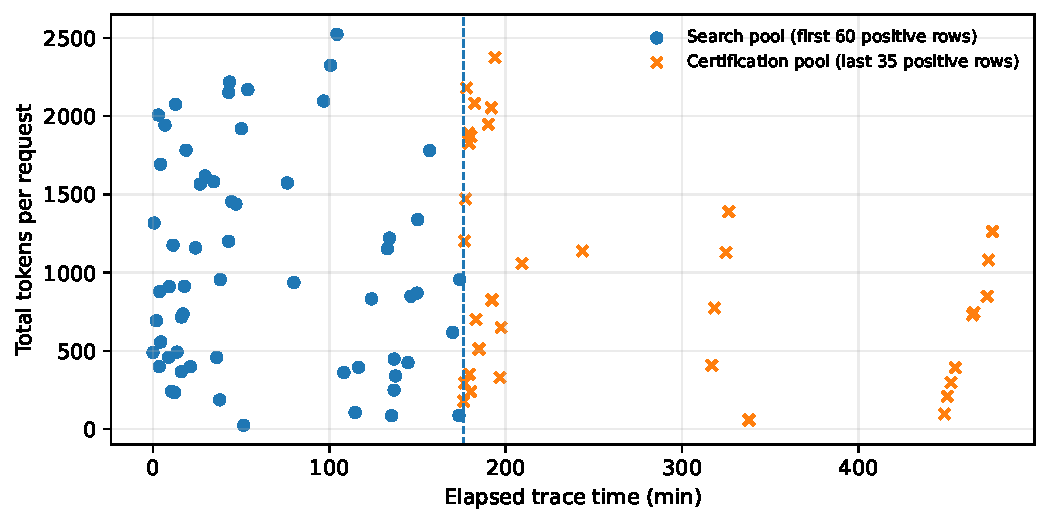
\includegraphics[width=.86\linewidth]{fig_v11_trace_slice.pdf}
\caption{The compact BurstGPT slice used in the original locked trace-derived study. It consists of the first 100 chronological rows of the official \texttt{BurstGPT\_1.csv} release; the chronological division is fixed at 60 positive-token records for search and 35 for certification. Privacy labels and block-bootstrap replays are synthetic.}
\label{fig:trace-slice}
\end{figure}

\subsection{Exploratory operating-envelope analysis and separately locked confirmation}
\label{sec:frontierdesign}

The universal strict-study abstention motivated a post hoc exploratory extension that is reported separately from the locked V11 result. Campaign~1 exhaustively evaluates all 190 policies in each of the 12 original trace-derived scenarios using 150 later-pool replays per policy, for 2,280 policy--scenario audits. Campaign~2 varies offered load, local capacity, activation delay, and selected joint capacity--load combinations. It covers 549 scenario--configuration batches, representing 325 distinct physical parameter settings; every batch evaluates all 190 policies with 150 certification replays. Campaign~3 evaluates certification stability from prefixes of 50, 100, 150, 300, 600, and 1,200 fresh replays at the original point, a feasibility boundary, a safer interior point, and a harder neighboring point. All tested configurations, including failures, are retained. These campaigns diagnose feasibility and evidence requirements; they are not prospective deployment certificates.

After the exploratory frontier was complete, one common interior point was fixed before new result generation: $K=40$ and $\rho=0.05$. Six physical scenarios cross $q_H\in\{0.20,0.50,0.80\}$ with $\tau\in\{0.5,2.0\}$. DR-BGS and guarded GP each use ten fresh search-initialization labels per scenario, while exhaustive training selection supplies one reference nomination per scenario. Every nominated policy is tested on two disjoint batches of 1,200 later-pool replays using the unchanged 2\%/5\% limits, 10\% violation-risk budget, and familywise 5\% error allocation. Confirmation requires both batches to certify. Repeated initialization labels that nominate the same policy within a scenario are treated as duplicates in inferential summaries. A first execution attempt stopped before result generation because some seed integers exceeded NumPy's permitted range; only the invalid seed values were amended, and the failed log, original lock, amended lock, and successful outputs are archived.

\subsection{Separately locked seven-day trace robustness replication}
\label{sec:v15design}

To test whether the compact trace basis drives the main conclusions, a separate protocol was locked before a larger-slice result generation. The source is the official \texttt{BurstGPT\_1.csv} file (1,429,737 rows; SHA-256 \texttt{46fc9480\allowbreak ef0b748e\allowbreak cb2b51d5\allowbreak 12ff08c1\allowbreak 96b03178\allowbreak 2cbe6f78\allowbreak e28044d7\allowbreak 68e86d5a}). The robustness window is defined by elapsed trace time rather than a round row count: timestamps from 0 to 604,800 s. Positive-token rows in the first five days form the search pool ($n=11{,}810$), while positive-token rows from days five through seven form the later certification pool ($n=6{,}086$). This expands the two pools by roughly two orders of magnitude while preserving a multi-day chronological separation.

The replay transformation, block length eight, 560 requests per replay, token-to-pressure mapping, privacy-label generator, 190-policy space, and absolute 2\%/5\% gate are unchanged. The high-load replication repeats all 12 original $(\rho,q_H,\tau)$ scenarios, builds 12-replication search surfaces, evaluates every policy with 150 later-pool replays, and compares DR-BGS and guarded GP under five initializations. The low-load replication fixes $K=40$ and $\rho=0.05$, crosses the same three privacy fractions and two activation delays, uses ten search initializations per method, and requires each distinct nomination to pass two disjoint 1,200-replay batches. The protocol, configuration, trace subset, provenance record, execution code, and hashes were locked before result generation. Exact binomial bounds remain conditional on independent replays from the declared generator; the additional replay count does not create new observations of the real workload distribution.

\subsection{Policy-space scaling}

An exploratory scaling experiment uses $q\in\{19,31,51\}$, corresponding to 190, 496, and 1,326 policies. Three representative scenarios are exhaustively evaluated at each resolution using six training and ten holdout replications per policy. DR-BGS retains a fixed 20-policy high-fidelity budget. This experiment measures evaluated fraction, work reduction, and decision loss; it is a scaling check rather than a second reliability study.

\subsection{Pareto and minimax-regret analysis}

The holdout metrics $(W,B_H,B_L,R_C)$ are normalized within each scenario. A simplex grid of 286 weight vectors with step 0.1, augmented by equal weights, produces 287 stakeholder profiles. For policy $a$ and weight $w$, let $C_w(a)$ be the normalized weighted cost and $C_w^\star$ its profile optimum. The robust policy is
\[
a_{\rm MR}\in\arg\min_{a\in\Aset_{19}}
\max_{w\in\mathcal W}[C_w(a)-C_w^\star].
\]
We report Pareto-set size, distinct profile optima, maximum min--max-normalized additive regret of the equal-weight and minimax-regret policies, and the equal-weight penalty paid by the robust compromise. The analysis uses 95 policy surfaces: the original 36 plus the 59-case Latin-hypercube stress set. Minimax regret is used as a decision-robustness criterion, not as a claim that one stakeholder profile is objectively correct \cite{groetzner2022regret}.

\subsection{Use of generative-AI tools in the research workflow}
Generative-AI tools assisted with language editing, LaTeX organization, drafting and reviewing Python code, and cross-file consistency checks. They did not replace the archived simulation runs or the authors' verification of the mathematical model, numerical outputs, references, and interpretation. All scripts used for reported results were rerun in the archived environment; result files, protocol files, and audit outputs were checked by the authors. Product details and the authors' responsibility statement appear in the Acknowledgements.

\section{Results}
\label{sec:results}

\subsection{Reproducibility audit and low-fidelity verification}

A fresh-room replay reproduced the archived scenario definitions, stationary curves, jump curves, and verification tables. The audit corrected four material defects before the hysteresis campaign: admitted-workload rates had used mean jump size times acceptance probability instead of truncated first moments; low-privacy overflow before activation had been counted as immediate cloud service; jump-selected policies had been selected and evaluated on the same streams; and common random numbers were not fully aligned across policies. All reported results use corrected semantics and independent training/holdout streams.

A post-study horizon and warm-up sensitivity audit used three representative scenarios (F01, R07, and V01), the exhaustive-training policy and a fixed deadband in each scenario, and 100 common-random-number replications per setting. Paired comparisons between the default 1,200/300 holdout horizon/warm-up and a 4,800/1,200 setting had 95\% confidence intervals containing zero in all six cases. On the 4,800-unit horizon, increasing warm-up from 300 to 1,200 changed the mean objective by at most 0.18\%. This limited diagnostic supports the chosen warm-up but is not a general steady-state proof.

At the selected two-threshold policies, the 321-point stationary solver has maximum probability-mass error $2.22\times10^{-16}$, maximum residual $1.43\times10^{-12}$, and nonnegative stationary probabilities. Doubling to 641 points changes the objective by 0.49\% in the median, 0.97\% at the 90th percentile, and 3.07\% at maximum. The main limitation is model fidelity: pooled median and 90th-percentile absolute errors for the principal metrics are 24.3\% and 64.1\%. These values were recomputed from the archived 36-scenario surfaces at the diffusion-selected policy using the 321-point stationary solver.

\begin{figure}[t]
\centering
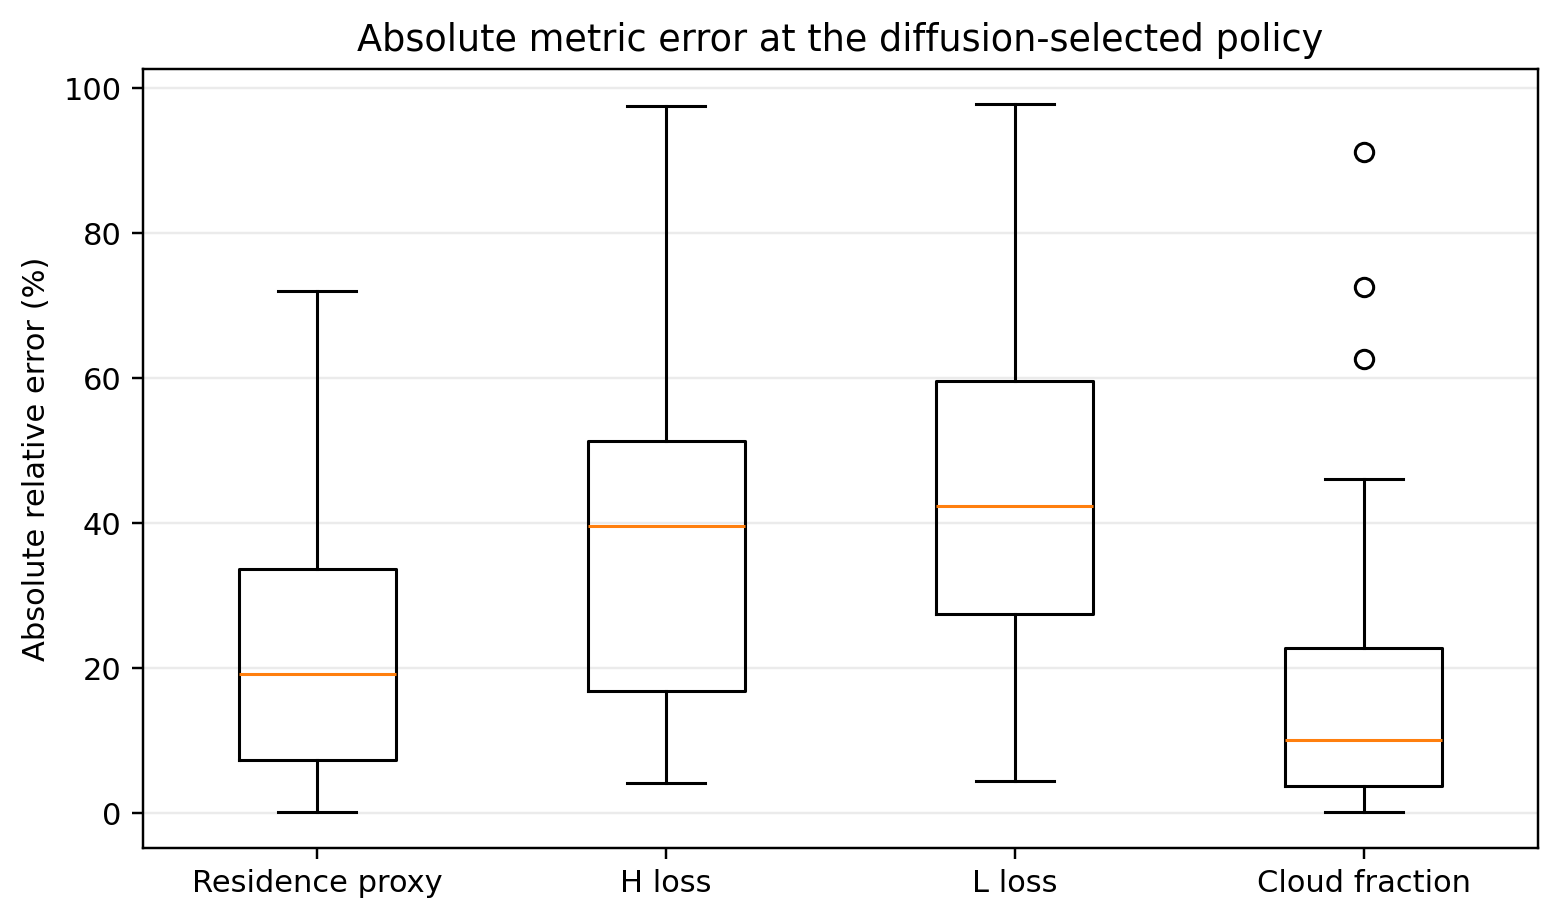
\includegraphics[width=.82\linewidth]{fig_audited_metric_errors.png}
\caption{Absolute metric errors of the diffusion surrogate at the diffusion-selected policy, recomputed from the archived 36-scenario surfaces with the 321-point stationary solver. The low-fidelity model is used as a prior, not as the final admission-risk estimator.}
\label{fig:metricerrors}
\end{figure}

\subsection{Equal-budget optimizer comparison and component ablation}

Table~\ref{tab:optimizers} compares the methods at a fixed budget of 20 high-fidelity policies, each with 20 training replications. DR-BGS and the guarded-GP ablation keep all 180 scenario--initialization runs within 1\% of the exhaustive training-selection workflow. DR-BGS has the smaller worst observed excess (0.348\% versus 0.878\%) and a slightly higher exact recovery rate (88.89\% versus 86.11\%). Standard GP Bayesian optimization has a 7.22\% maximum excess. A breadth-first two-stage ranking-and-selection procedure spends the same 400 training replications by sampling all 190 policies twice and then resampling a ten-policy shortlist; it is within 1\% in 70.56\% of runs and has 11.67\% maximum excess. In this benchmark, this broad-but-shallow allocation does not match the structured searches.

\begin{table}[t]
\centering
\small
\caption{Fixed 20-policy high-fidelity budget on 36 scenarios. Stochastic methods use five fixed initializations. ``Exhaustive'' denotes exhaustive training selection evaluated on holdout.}
\label{tab:optimizers}
\resizebox{\linewidth}{!}{%
\begin{tabular}{lrrr}
\toprule
Method & Runs within 1\% & Runs within 5\% & Maximum excess\\
\midrule
High-fidelity local search & 13.89\% & 44.44\% & 34.02\%\\
Random subset R\&S & 56.11\% & 87.22\% & 13.26\%\\
Breadth-first two-stage R\&S & 70.56\% & 96.11\% & 11.67\%\\
Diffusion top-20 & 86.11\% & 91.67\% & 9.97\%\\
Standard GP Bayesian optimization & 95.56\% & 98.89\% & 7.22\%\\
Guarded GP, no diffusion residual & 100.00\% & 100.00\% & 0.878\%\\
DR-BGS & 100.00\% & 100.00\% & 0.348\%\\
\bottomrule
\end{tabular}%
}
\end{table}

\begin{figure}[t]
\centering
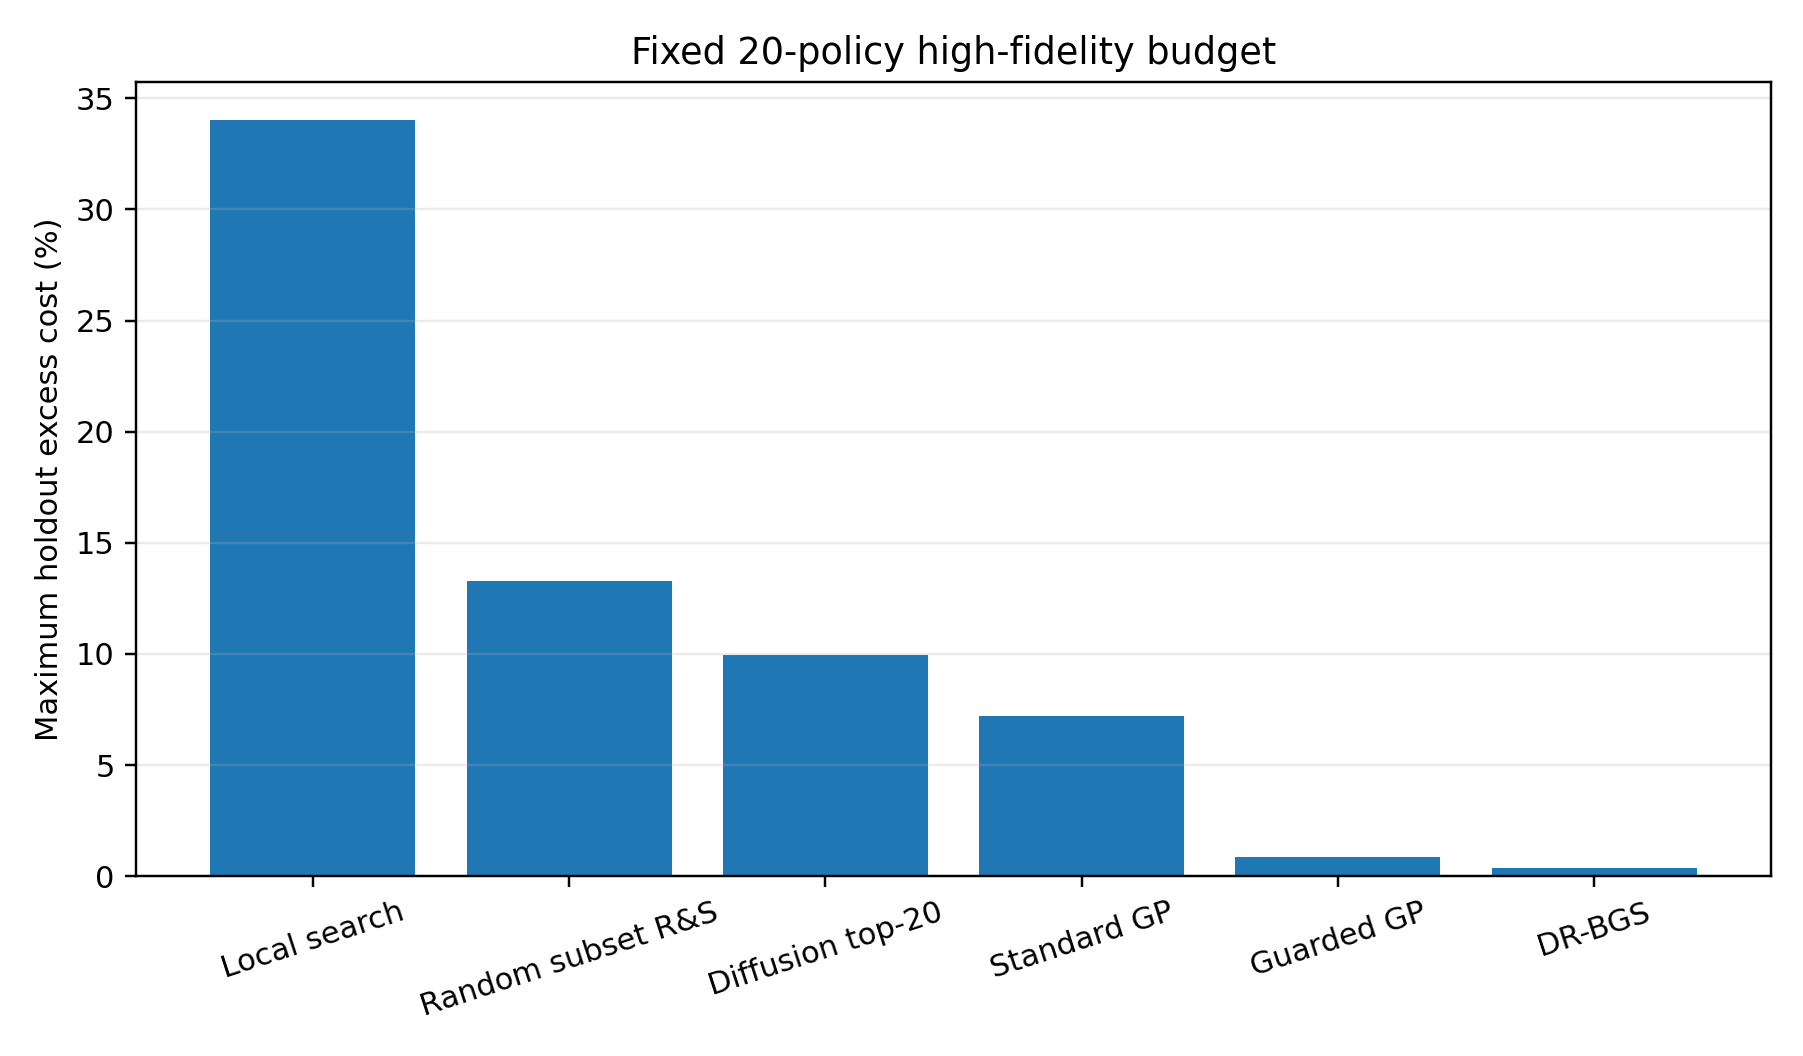
\includegraphics[width=.88\linewidth]{fig_v8_optimizer_comparison.png}
\caption{Worst observed holdout excess under a fixed 20-policy high-fidelity budget.}
\label{fig:optimizercomparison}
\end{figure}

The ablation limits the interpretation of the residual model. At a budget of 12 policies, the guarded GP has a lower maximum excess than DR-BGS (0.878\% versus 1.07\%). At 20 policies, residual calibration reduces the maximum from 0.878\% to 0.348\%. An unguarded residual GP still has a 7.22\% maximum at that budget. The structural anchors account for most of the reliability; the diffusion residual provides a smaller and budget-dependent reduction in tail loss.

\begin{figure}[t]
\centering
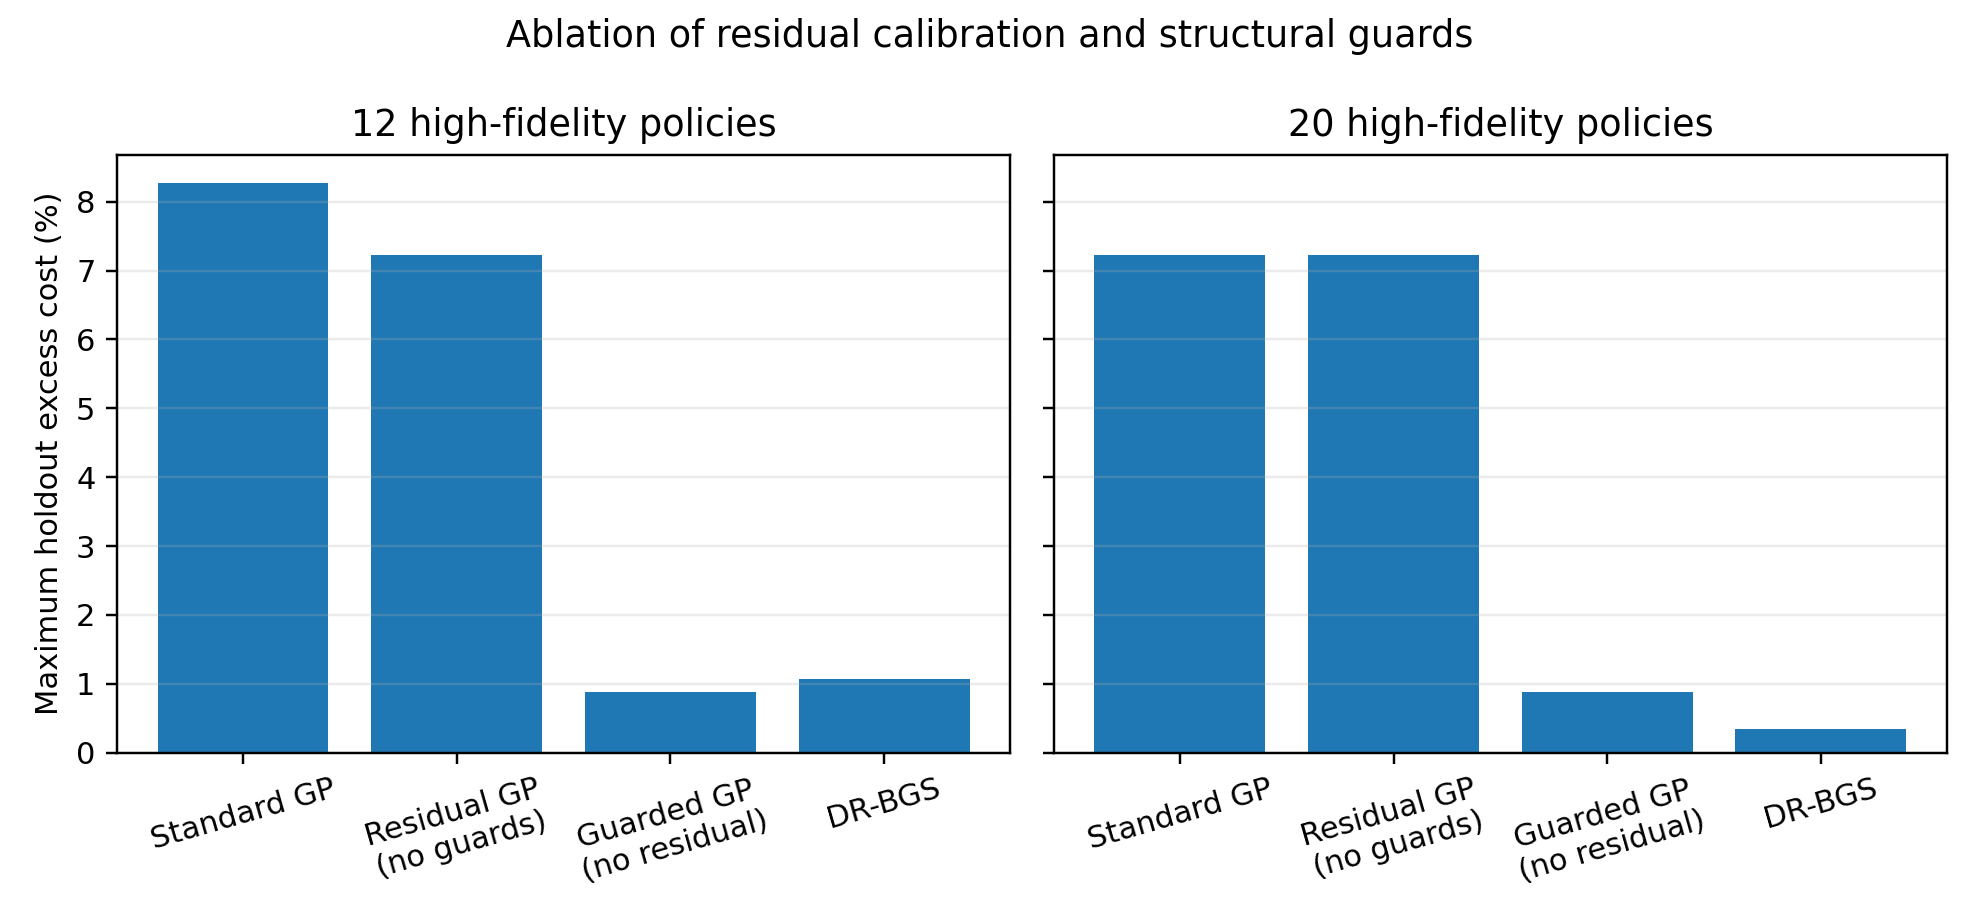
\includegraphics[width=.9\linewidth]{fig_v8_component_ablation.png}
\caption{Ablation of structural guards and diffusion-residual calibration at 12- and 20-policy budgets.}
\label{fig:componentablation}
\end{figure}

MIGR-H remains within 5\% in all 36 scenarios but explores about 36.7 policies on average. At the 20-policy budget, the Bayesian guarded methods achieve similar or better decision quality with less high-fidelity work.

\subsection{Independent scenario evidence}

The two older 59-scenario sets remain descriptive because their archive does
not contain an immutable study lock preceding generation. Their maximum
excesses are 0.638\% and 0.306\%.

The first internally locked study is more demanding. Under its 1\% primary
criterion, 57 of 59 scenarios succeed for all five initializations. The exact
one-sided 95\% lower confidence bound for scenario-level success is 89.71\%.
The two retained failures have maximum excesses of 1.15\% and 3.49\%; all 295
runs are within 5\%. The primary criterion does not pass at a level
that would support a 95\% reliability statement. This negative result is kept
in the release.

\begin{table}[t]
\centering
\small
\caption{Independent 59-scenario evidence. A scenario succeeds only when all five fixed initializations satisfy the stated excess-cost threshold.}
\label{tab:locked}
\resizebox{\linewidth}{!}{%
\begin{tabular}{lrrrr}
\toprule
Study & Locked threshold & Successful scenarios & One-sided 95\% lower bound & Maximum excess\\
\midrule
V9 strict study & 1\% & 57/59 & 89.71\% & 3.49\%\\
V9B follow-up study & 5\% & 59/59 & 95.05\% & 0.941\%\\
\bottomrule
\end{tabular}%
}
\end{table}

The follow-up study was internally locked before its own generation with a 5\% practical indifference threshold. All 59 scenarios satisfy the primary criterion for all five initializations, which gives a one-sided 95\% Clopper--Pearson lower bound of 95.05\%. All 295 runs also fall within 1\%, and the maximum excess is 0.941\%. The study was designed after the strict-study result and is therefore reported as follow-up evidence, not as a retroactive repair or independently preregistered confirmation.

\subsection{Trace-derived risk audit}
\label{sec:traceresults}

The chronological trace shift changes the decision problem materially. Under the strict absolute certificate, neither DR-BGS nor the same-anchor guarded GP certifies any of the 60 method--initialization runs. For DR-BGS, mean protected blocking across certification batches ranges from 12.7\% to 28.8\% over the 12 scenarios, well above the 2\% replay threshold. Eligible blocking is also above its 5\% limit in most scenarios. The largest exact upper risk bound is at least 0.985 in every scenario, compared with the prespecified budget of 0.10. Figure~\ref{fig:absolute-cert} displays the resulting abstention.

\begin{figure}[t]
\centering
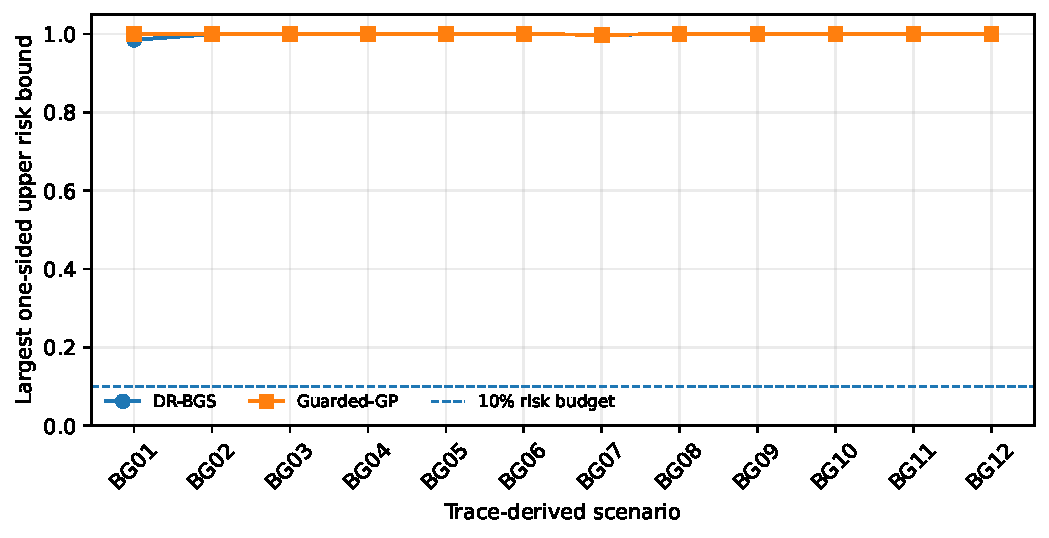
\includegraphics[width=.86\linewidth]{fig_v11_absolute_slo_certification.pdf}
\caption{Strict absolute-SLO certification on the later BurstGPT-derived pool. Each point is the largest of the protected- and eligible-blocking risk upper bounds for one scenario and method, maximized over five initializations. The dashed line is the 10\% risk budget. Every run abstains.}
\label{fig:absolute-cert}
\end{figure}

Universal abstention is a negative result, not a safety guarantee. It means that, under the declared pressure mapping, capacity, trace resampling, and strict limits, independent simulation does not support deployment of any nominated policy. The search-stage training surface can look feasible while the later pool is not. This is precisely the failure mode the independent gate is intended to expose.

The separately locked independent-seed noninferiority follow-up asks a narrower retrospective question: is the nomination materially worse than exhaustive training selection on paired later-pool replays? DR-BGS is certified in 50 of 60 runs (83.3\%) and abstains in 10; the guarded GP is certified in 33 of 60 (55.0\%) and abstains in 27. DR-BGS certifies all five initializations in 10 of 12 scenarios, while the guarded GP does so in five. In this experiment every certified run also recovers the exhaustive training-selected policy exactly. The certificate therefore identifies agreement with the expensive reference and abstains on the nonmatching cases; it does not prove that an unseen nonmatching policy is near-optimal.

\begin{table}[t]
\centering
\caption{Trace-derived risk-audit results. Absolute certification tests declared blocking-risk targets without an exhaustive reference. Noninferiority certification is a retrospective paired comparison with exhaustive training selection.}
\label{tab:trace-risk}
\small
\begin{tabular}{lccc}
\toprule
Method & Absolute SLO & Paired noninf. & Work reduction \\
\midrule
DR-BGS & 0/60 & 50/60 (83.3\%) & 83.95\% \\
Guarded GP & 0/60 & 33/60 (55.0\%) & 83.95\% \\
\bottomrule
\end{tabular}
\end{table}

\begin{figure}[t]
\centering
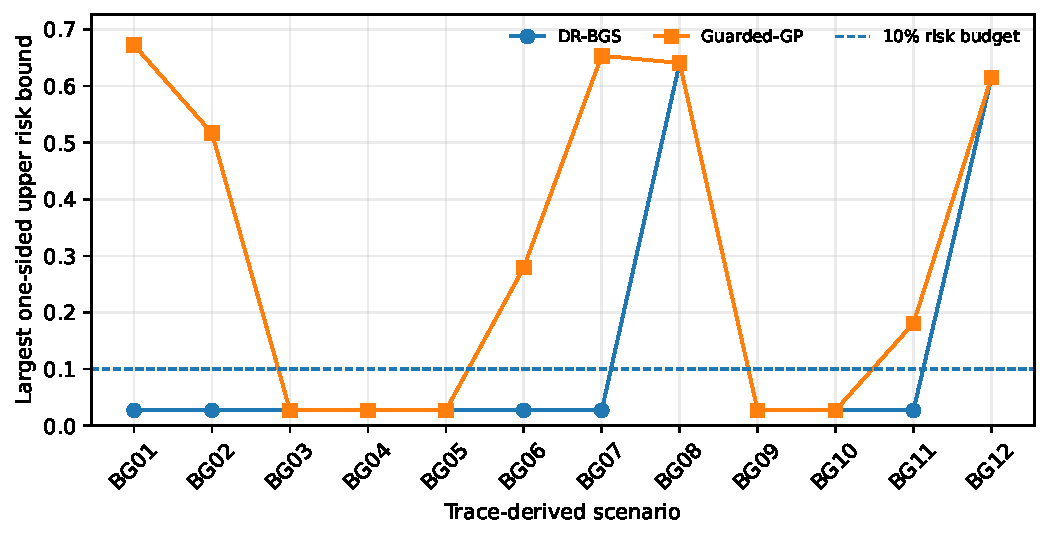
\includegraphics[width=.86\linewidth]{fig_v11_noninferiority_certification.pdf}
\caption{Paired noninferiority audit against exhaustive training selection. Each point is the largest of three one-sided exact risk bounds, maximized over five initializations. Values above 0.10 lead to abstention.}
\label{fig:noninferiority-cert}
\end{figure}

On the 30-replication trace holdout used for ordinary decision loss, DR-BGS has median and 90th-percentile excess of zero and maximum excess 14.99\%; the guarded GP has median zero, 90th percentile 7.26\%, and the same maximum. These tails are substantially worse than the original synthetic benchmark. The trace slice is small, but the result establishes that the later temporal segment is not interchangeable with the search segment under the declared replay transformation.

\subsection{Operating-envelope diagnosis and separately locked low-load confirmation}
\label{sec:frontierresults}

The exhaustive audit shows that the original absolute-SLO abstention is not merely a nomination failure. At $K=40$ and $\rho\in\{0.70,0.90\}$, none of the 2,280 policy--scenario combinations passes the unchanged 2\%/5\% gate, and no policy meets both limits even in its sample means. The jointly least-bad policies still have protected blocking of 11.12\%--28.28\% and eligible blocking of 5.99\%--19.79\%. Increasing the evidence batch to 1,200 replays produces no certification for DR-BGS, guarded GP, exhaustive training selection, or the risk-screen diagnostic. The original failure is therefore operational under the declared policy family and replay generator, not a shortage of certification replications.

The exploratory engineering sweeps identify no inexpensive repair. At baseline capacity, the highest certifiable load ratio is 0.05 or 0.075 depending on scenario, and no load-only case certifies at $\rho\ge0.10$. At the original loads, capacity-only increases through $K=240$ certify only BG01 at $K=200$ and BG03 at $K=240$; the other ten scenarios remain uncertified. Reducing activation delay to 0.10 certifies no scenario. Among the 38 scenario--configuration batches that contain at least one certifiable policy, DR-BGS certifies 135 of 190 nominations and guarded GP 140 of 190. The frontier therefore does not establish DR-BGS superiority under shifted operating conditions; it identifies when a separate risk gate can support either method's nomination.

The separately locked low-load study confirms that the gate can issue stable positive decisions inside a feasible regime. At $K=40$ and $\rho=0.05$, all six unique DR-BGS scenario--policy pairs pass both disjoint 1,200-replay batches. The same is true for all twenty unique guarded-GP pairs and all six exhaustive-training pairs. These method-specific counts sum to 32; after cross-method deduplication, they represent 31 distinct scenario--policy pairs because DR-BGS and exhaustive training select the same policy in scenario C06. All 31 pass both batches, with no batch-to-batch reversal; the largest reported one-sided upper risk bound is 0.01419, below the 0.10 budget. The 60/60 DR-BGS initialization labels are not treated as independent physical validations because all ten labels within each scenario nominate the same policy. Relative to the original $\rho=0.70/0.90$ settings, $\rho=0.05$ represents a 92.9\%--94.4\% load reduction. The result validates gate functionality in an interior regime but is not a practical deployment recommendation.

\begin{table}[t]
\centering
\small
\caption{Operating-envelope diagnosis and duplicate-aware low-load confirmation. Exploratory rows diagnose the strict gate; the final row group uses a separately locked fresh-seed study.}
\label{tab:operating-envelope}
\begin{tabular}{p{0.27\linewidth}p{0.18\linewidth}p{0.41\linewidth}}
\toprule
Regime or change & Evaluator & Outcome \\
\midrule
Original $K=40$, $\rho=0.70/0.90$ & All 190 policies & 0/2,280 policy--scenario pairs certified \\
Activation delay reduced to 0.10 & All 190 policies & 0/12 scenarios certified \\
Capacity increased through $K=240$ & All 190 policies & 2/12 scenarios certified \\
Load reduced at $K=40$ & All 190 policies & Certification only at $\rho\le0.05$ or $0.075$; none at $\rho\ge0.10$ \\
\midrule
Locked $K=40$, $\rho=0.05$ & DR-BGS & 6/6 unique pairs pass both batches \\
Locked $K=40$, $\rho=0.05$ & Guarded GP & 20/20 unique pairs pass both batches \\
Locked $K=40$, $\rho=0.05$ & Exhaustive training & 6/6 unique pairs pass both batches \\
\bottomrule
\end{tabular}
\end{table}

\subsection{Seven-day trace robustness results}
\label{sec:v15results}

The larger chronological window reproduces both sides of the original finding. In the 12 high-load scenarios, none of the 2,280 exhaustive policy--scenario combinations passes the unchanged absolute gate. DR-BGS, guarded GP, and exhaustive training therefore certify 0/60, 0/60, and 0/12 nomination labels, respectively. The jointly least-bad policy in each scenario still exceeds at least one sample-mean blocking limit: protected blocking ranges from 5.37\% to 32.09\%, and eligible blocking from 2.11\% to 18.92\% across the twelve jointly selected diagnostic policies. The smallest largest exact upper risk bound is 0.855, far above the 0.10 budget.

At the fixed low-load point, all six distinct DR-BGS scenario--policy pairs, all twelve guarded-GP pairs, and all six exhaustive-training pairs pass both disjoint 1,200-replay batches. The method-specific counts sum to 24, but cross-method deduplication leaves 18 distinct scenario--policy pairs; all 18 are confirmed, with no batch-to-batch reversal. The largest upper risk bound across methods and batches is 0.00307. As in V13, repeated initialization labels are not treated as independent physical validations.

The seven-day replication therefore removes the concern that the qualitative high-load/low-load contrast is an artifact of only 95 positive-token records. It does not remove model risk: privacy labels, pressure mapping, target load, and replay construction remain synthetic, and the exact bounds describe the declared generator rather than the live BurstGPT workload.

\begin{figure}[t]
\centering
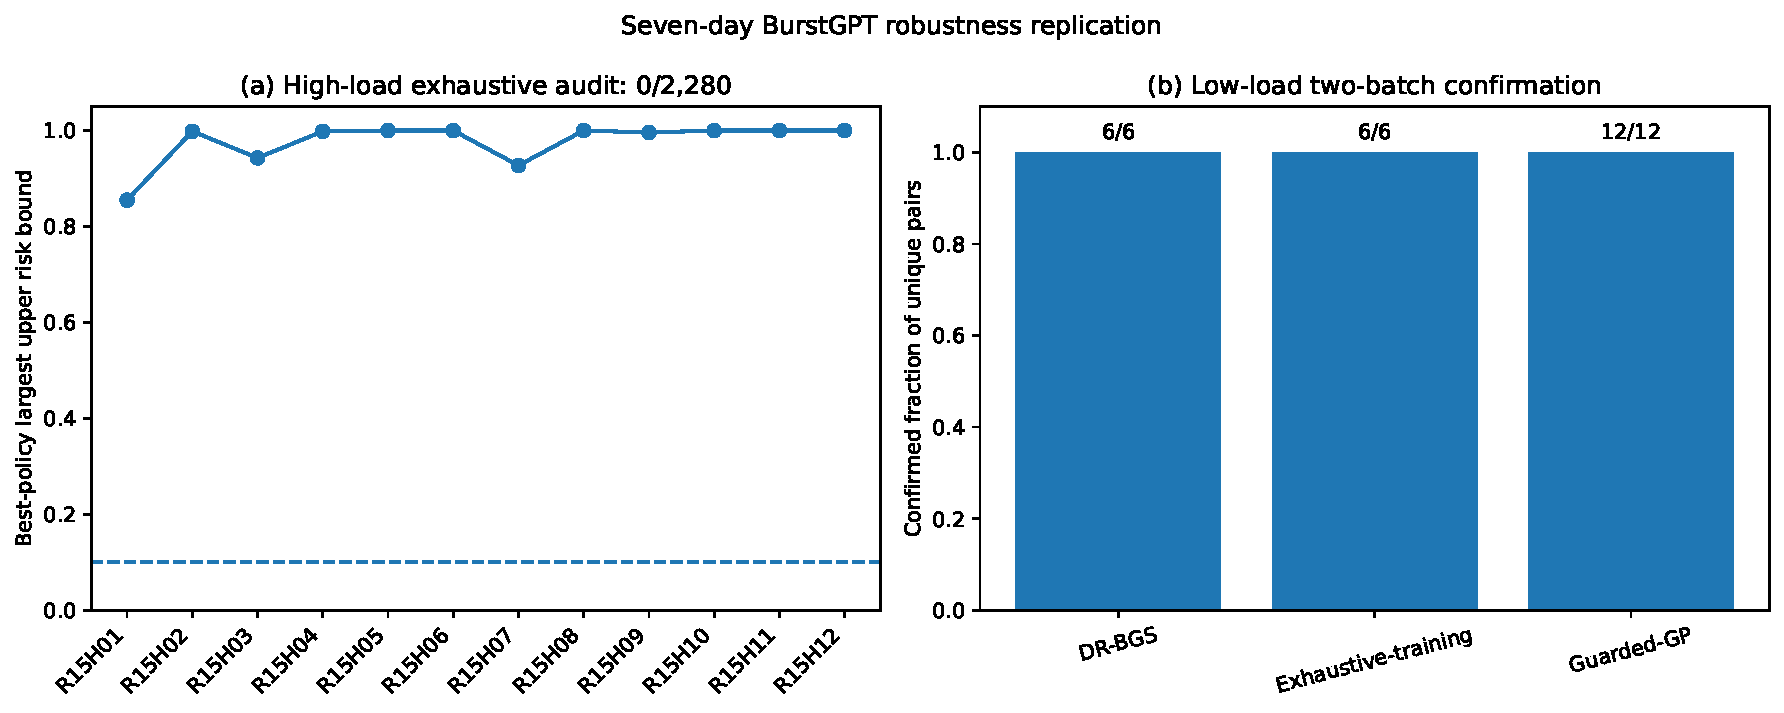
\includegraphics[width=.98\linewidth]{fig_v15_seven_day_robustness.pdf}
\caption{Separately locked seven-day BurstGPT robustness replication. (a) For each high-load scenario, the point is the lowest attainable largest exact upper risk bound among all 190 policies; every value exceeds the 0.10 budget. (b) At $K=40$, $\rho=0.05$, every unique method-specific scenario--policy pair passes both disjoint 1,200-replay batches. Method-specific pairs overlap across methods, leaving 18 cross-method-distinct pairs.}
\label{fig:v15-robustness}
\end{figure}

\subsection{Policy-space scaling}

Table~\ref{tab:scaling} reports an exploratory dense-grid test. DR-BGS evaluates 20 policies at every resolution, so the evaluated fraction falls from 10.53\% at 190 policies to 1.51\% at 1,326 policies. Mean high-fidelity replication reduction rises from 88.70\% to 98.37\%. Exact recovery is not monotone because the denser grids contain broad, near-tied basins. Relative to exhaustive training selection, the maximum holdout excess is 5.96\%, 3.15\%, and 0.00\% at the three resolutions. Only three scenarios and reduced replication counts are used at each resolution, so the result is a computational scaling check rather than a reliability study.

\begin{table}[t]
\centering
\small
\caption{Exploratory scaling of DR-BGS with a fixed 20-policy high-fidelity budget.}
\label{tab:scaling}
\begin{tabular}{rrrrr}
\toprule
Policies & Evaluated fraction & Work saved & Median excess & Maximum excess\\
\midrule
190 & 10.53\% & 88.70\% & 1.45\% & 5.96\%\\
496 & 4.03\% & 95.65\% & 0.10\% & 3.15\%\\
1,326 & 1.51\% & 98.37\% & 0.00\% & 0.00\%\\
\bottomrule
\end{tabular}
\end{table}

\begin{figure}[t]
\centering
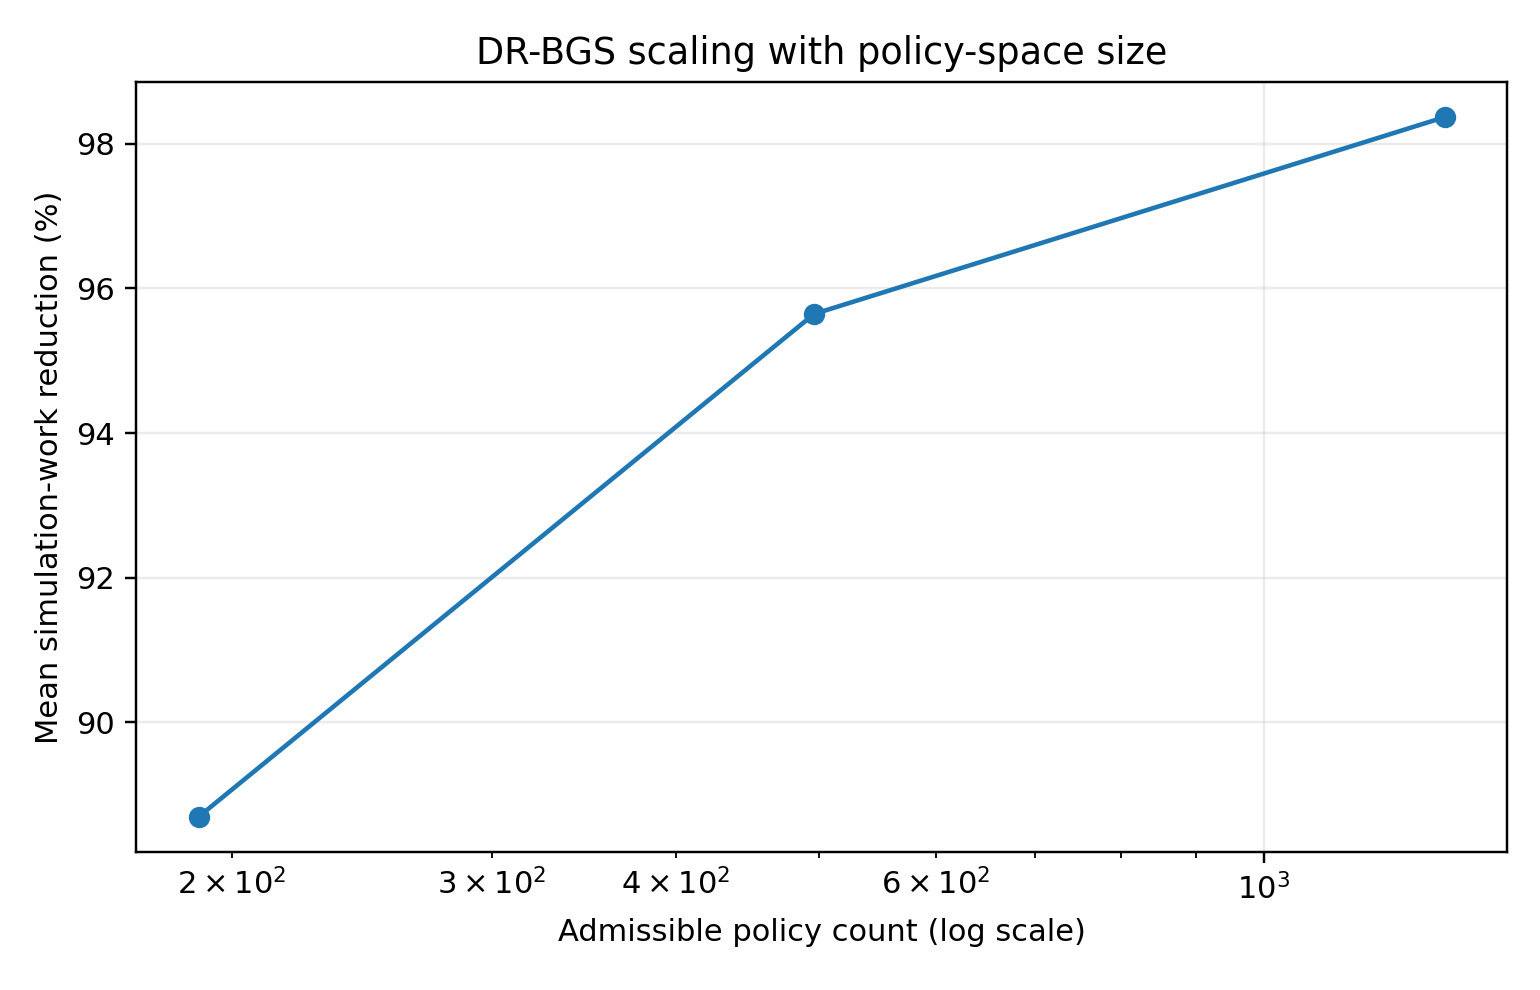
\includegraphics[width=.78\linewidth]{fig_v7_scaling.png}
\caption{Simulation-work reduction as the triangular hysteresis grid expands.}
\label{fig:scaling}
\end{figure}

\subsection{Practical policy baselines and activation delay}

Using one prespecified DR-BGS initialization, the selected policies improve the median holdout objective by 30.96\% relative to local-only execution, 13.28\% relative to $(0.5K,0.5K)$, and 11.79\% relative to the fixed $(0.5K,0.4K)$ deadband; DR-BGS is better in all 36 scenarios for these comparisons. Against the strongest trained diagonal policy, the median change is $-0.38$\% and DR-BGS is better in 41.67\% of cases, consistent with the modest incremental value of a second threshold.

A delay-aware diffusion design evaluated under the actual-delay jump model improves over a near-instantaneous design by 3.04\% in the development median, 12.82\% at the 90th percentile, and 17.69\% at maximum. Activation delay is not uniformly decisive, but ignoring it materially changes the policy in specific regimes.

\subsection{Incremental value of hysteresis}

As a retrospective diagnostic using the complete holdout surfaces, the best strict-hysteresis policy improves over the best diagonal policy in 41.67\% of the original 36 scenarios. The median gain is zero, the 90th percentile is 1.03\%, and the maximum is 2.85\%. The expanded space is useful because it contains both policy classes and permits data-driven selection; the result does not support universal superiority of strict hysteresis.

\begin{figure}[t]
\centering
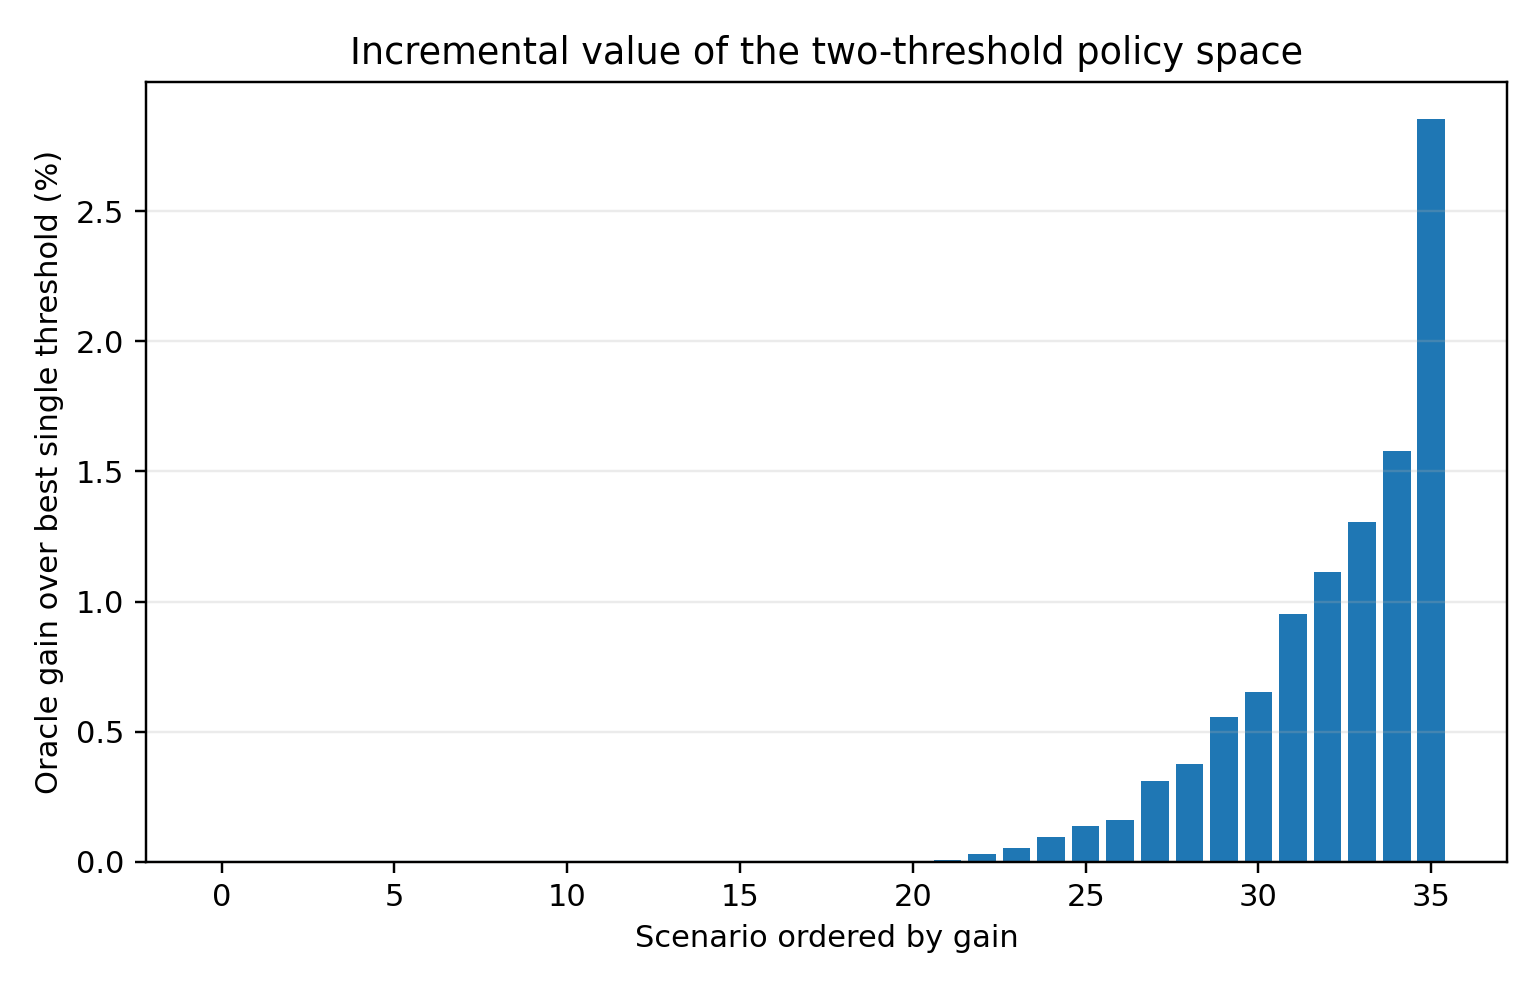
\includegraphics[width=.74\linewidth]{fig_v5_hysteresis_gain.png}
\caption{Incremental holdout-oracle gain from admitting a second threshold.}
\label{fig:hystgain}
\end{figure}

\subsection{Pareto and minimax-regret policy selection}

Across 95 scenarios and 287 weight profiles, the median Pareto set contains 118 of 190 policies and the median number of distinct profile-optimal policies is 13. The minimax-regret policy differs from the equal-weight policy in every scenario and is Pareto efficient in the point-estimate surfaces. Its median maximum min--max-normalized additive regret is 0.462, compared with 1.000 for the equal-weight policy, a median reduction of 52.63\%. The compromise pays a median normalized penalty of 0.174 under equal weights. This is a worst-profile trade-off: in the median scenario, the minimax policy is more than 5\% above the profile optimum for 83.62\% of weight profiles, compared with 19.51\% for the equal-weight policy.

\begin{figure}[t]
\centering
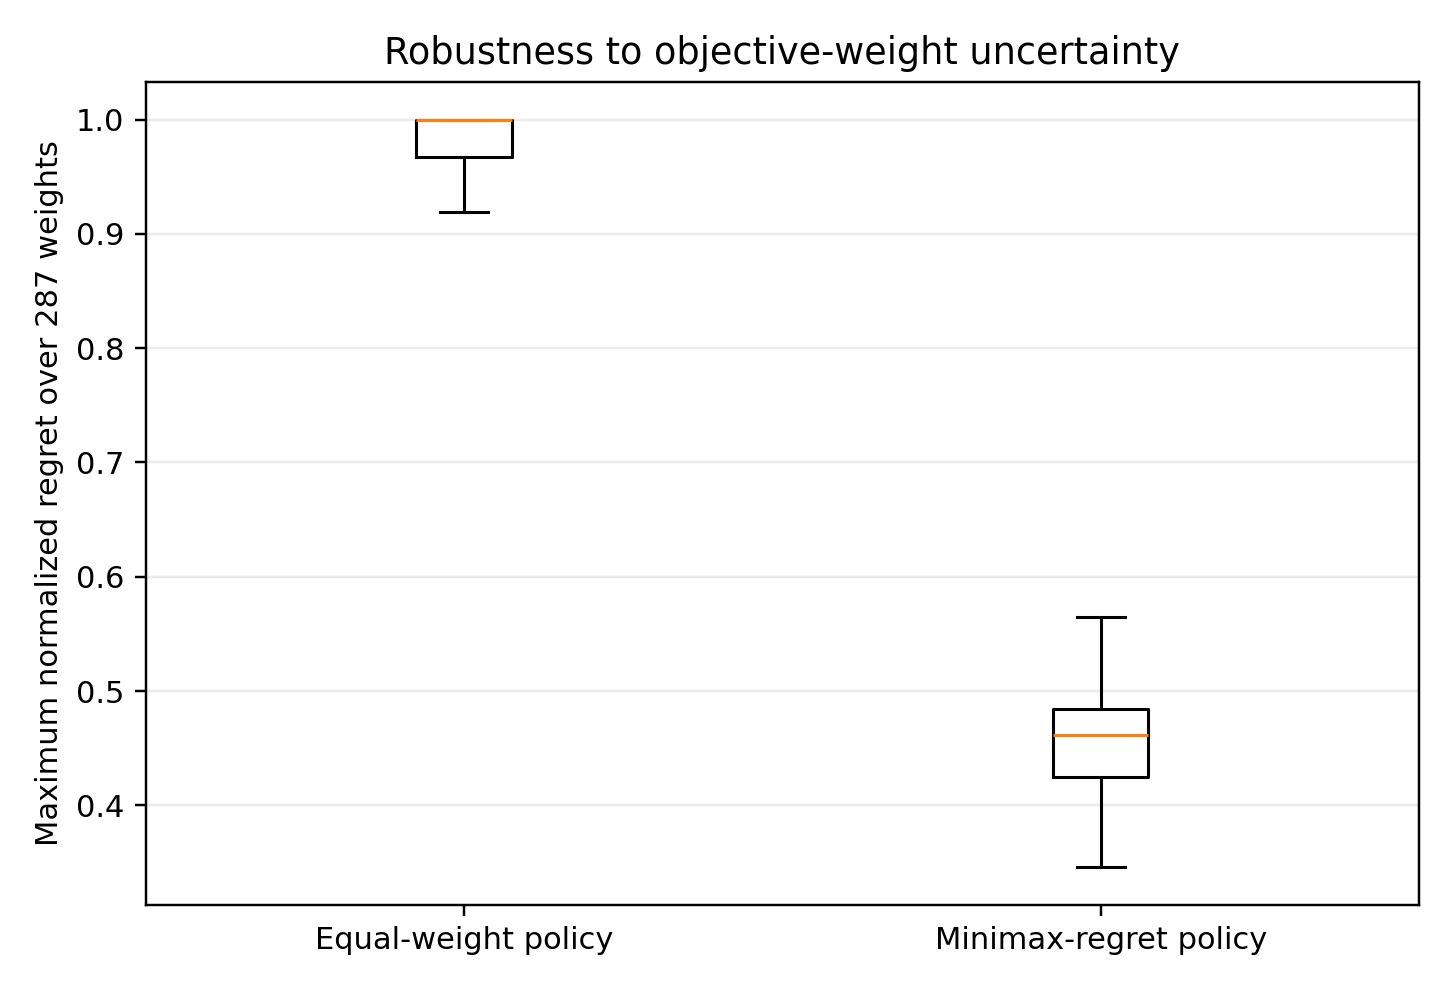
\includegraphics[width=.72\linewidth]{fig_v7_robust_regret.png}
\caption{Maximum normalized regret of equal-weight and minimax-regret policies over 287 stakeholder profiles.}
\label{fig:robustregret}
\end{figure}

\begin{figure}[t]
\centering
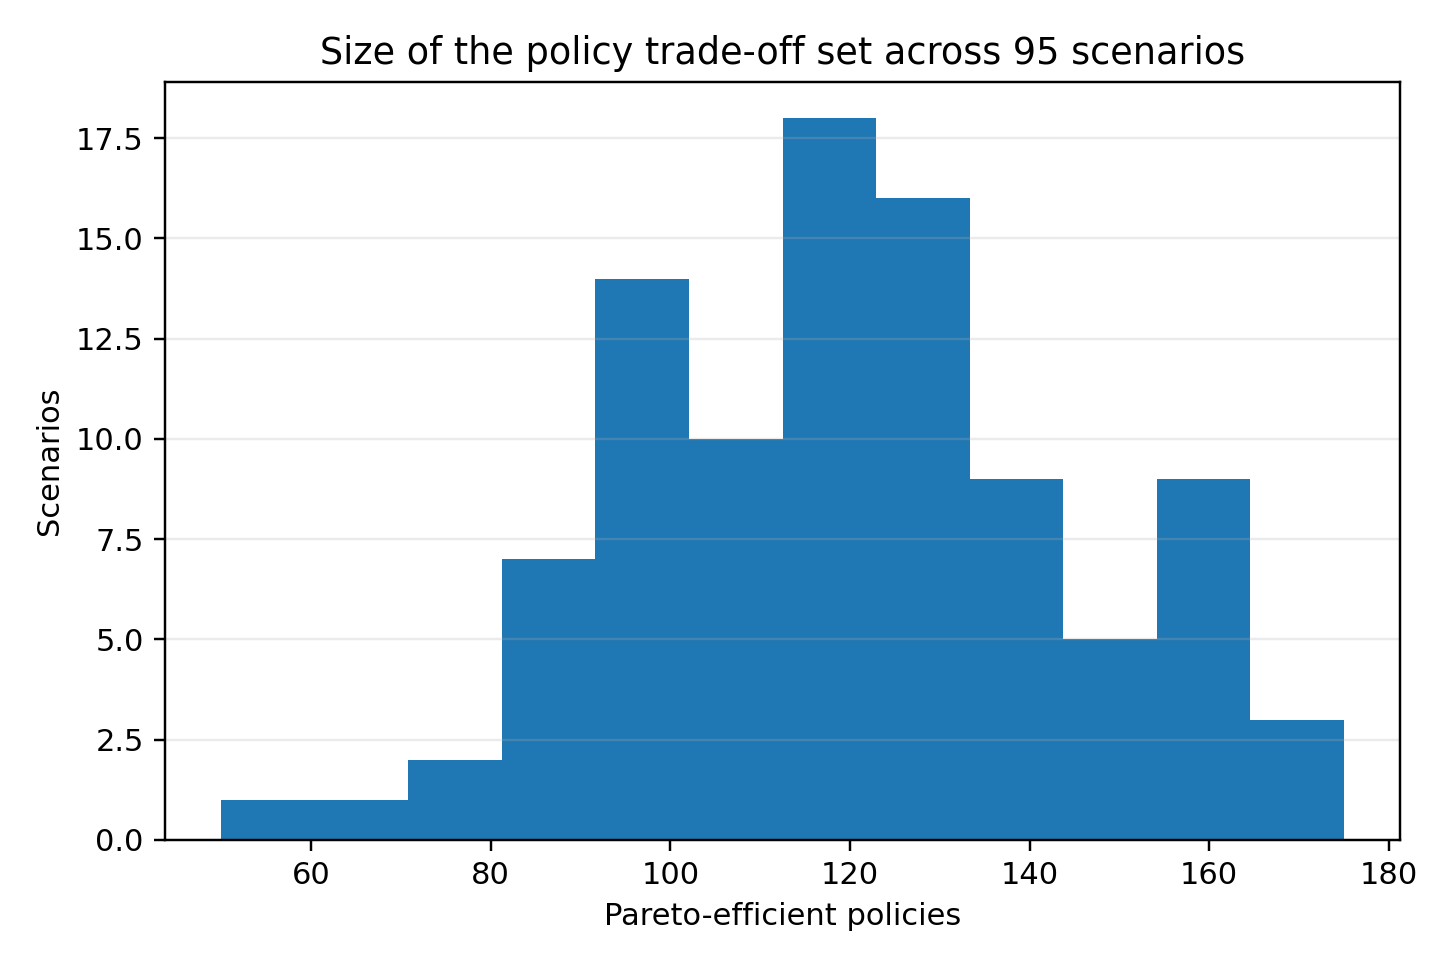
\includegraphics[width=.72\linewidth]{fig_v7_pareto_size.png}
\caption{Distribution of Pareto-set sizes across 95 scenarios.}
\label{fig:paretosize}
\end{figure}

\FloatBarrier
\FloatBarrier
\section{Empirical service-law grounding}
\label{sec:calibration}

The existing vLLM calibration uses Qwen2.5-7B on an RTX 3090 at six concurrency levels with direct cache telemetry. The exponential fit is
\[
\widehat\mu(z)=53.6138\exp(-0.034451z),
\]
with $R^2=0.9961$, RMSE 0.789 tokens/s, and leave-one-level-out RMSE 1.299 tokens/s. A 20,000-draw bootstrap gives a normalized observed-range sensitivity interval of 1.159--1.358. The simulation design covers a wider $\beta$ interval of 0.600--1.376 to include structural uncertainty. RTX 4090 and Mistral measurements are retained as qualitative checks because they used concurrency rather than identical direct cache telemetry.

\begin{figure}[t]
\centering

\includegraphics[width=.8\linewidth]{fig_calibration_service_fit.pdf}
\caption{Direct-telemetry service-law calibration used to define plausible low-fidelity parameter ranges.}
\label{fig:calibration}
\end{figure}

The hardware data calibrate the shape and range of the reduced-order model. They do not validate the 190-policy controller on a production serving system, and no such claim is made.

\section{Discussion and limitations}
\label{sec:discussion}

Four conclusions survive the combined evidence. First, structural boundary and diagonal coverage is the main reason the guarded searches avoid catastrophic failures on the synthetic benchmark. The diffusion residual improves the 20-policy worst case from 0.878\% to 0.348\%, but the advantage is budget-dependent and smaller than the effect of the guards.

Second, efficient nomination and operational feasibility are different questions. The chronological trace study exposes a severe distribution shift: policies that appear feasible on the first 60 records violate the declared limits on the later pool. Exhaustive evaluation of all 190 alternatives shows that no policy in the tested family is certifiable at the original $\rho=0.70/0.90$ operating points. Increasing the certification batch to 1,200 replays does not rescue those regimes. Universal abstention is therefore not merely conservative uncertainty around a potentially feasible nomination; under the declared simulator and policy family, it reflects an operationally infeasible region.

Third, the exploratory frontier and fresh-seed confirmation show that the absolute gate is capable of returning positive decisions. Faster activation alone does not suffice, and capacity-only expansion through six times baseline helps only two scenarios. Load reduction is the most consistent path to feasibility. At the separately locked $K=40$, $\rho=0.05$ point, every unique DR-BGS, guarded-GP, and exhaustive-training nomination passes two disjoint 1,200-replay batches. The seven-day trace replication independently reproduces this qualitative contrast: 0/2,280 high-load policy--scenario pairs certify, whereas all 18 cross-method-distinct low-load pairs pass both batches. This validates the gate's fail-safe structure across two trace bases. It does not show that the low-load point is economically attractive or that DR-BGS outperforms guarded GP there.

Fourth, the retrospective noninferiority audit remains useful but narrower. DR-BGS agrees with exhaustive training selection more often than the same-anchor GP under the trace-derived design, with 50/60 versus 33/60 certified labels. Because computing the reference requires exhaustive training evaluation, that result cannot serve as a deployable optimality guarantee. The absolute certificate is deployable in principle within the simulator, but positive certification requires the service configuration to operate inside a feasible envelope.

The trace evidence still has important limits. The original locked study uses 95 positive-token rows, and the robustness replication expands this to a fixed seven-day window with 17,896 positive-token rows; neither uses the complete 1,429,737-row \texttt{BurstGPT\_1.csv} file or the other BurstGPT releases. The larger window materially reduces dependence on a tiny viewer-sized slice, but moving-block bootstrap preserves only short local sequences and cannot establish full-corpus representativeness or reproduce all long-range seasonality. Timestamp gaps and token counts are trace-derived; privacy labels, pressure mapping, target load, and phase parameters remain synthetic. The risk bounds are conditional on independent replays from the declared generator. They are not bounds on a live production system.

The workload-pressure state is a reduced-order abstraction. The simulator omits scheduler-specific preemption, prefix sharing, network congestion, remote queueing, model-quality routing, and privacy-classifier error. The empirical service-law fit defines a plausible pressure-relief shape but does not validate the controller on hardware. Full-corpus trace replay, additional hardware environments, and live cloud--edge evaluation remain necessary. A live controller would also require online drift detection, explicit capacity planning, and a policy for what happens after abstention.

Finally, this paper does not propose a general safe or constrained Bayesian-optimization theorem. The GP does not enforce deployment constraints, and the exact risk gate does not make unsafe search evaluations safe. Its contribution is a problem-specific separation of mechanistic screening, high-fidelity nomination, operational-envelope diagnosis, and independent evidence gating, together with both retained failure and positive interior-regime confirmation.
\section{Conclusion}
\label{sec:conclusion}

DR-BGS allocates a limited compound-jump simulation budget over a 190-policy cloud-activation grid. On 36 exhaustive synthetic scenarios, 20 high-fidelity policies are sufficient for all 180 selections to remain within 1\% of exhaustive training selection on independent holdout streams, while reducing replications by 88.77\%. The guarded-GP ablation confirms that structural anchors contribute more than the diffusion residual.

The trace-derived extension changes the interpretation of that result. Under strict 2\% protected-blocking and 5\% eligible-blocking limits, the original high-load study certifies none of the 120 method runs. Exhaustive auditing then finds no certifiable policy among all 2,280 policy--scenario combinations, and larger certification batches do not alter the outcome. The failure is therefore tied to the operating regime and examined policy family rather than solely to search error or insufficient statistical evidence.

An exploratory frontier identifies the conditions under which the same gate becomes supportable. Load reduction is the most consistent mechanism; faster activation alone fails, and large capacity increases help only a small subset of scenarios. A separately locked fresh-seed confirmation at $K=40$, $\rho=0.05$ shows that every unique DR-BGS, guarded-GP, and exhaustive-training nomination passes two disjoint 1,200-replay batches. A further seven-day BurstGPT replication reproduces 0/2,280 high-load certifications and confirms all 18 cross-method-distinct low-load pairs. These positive results establish that the gate is not structurally incapable of certification, but the required 92.9\%--94.4\% load reduction makes the point an operating-envelope diagnostic rather than a deployment recommendation.

The practical workflow is therefore: use the mechanistic model and structural guards to nominate policies cheaply; diagnose whether the operating regime contains a certifiable alternative; base the final claim on independent high-fidelity evidence; and abstain when the target is unsupported. Full-corpus trace replay, additional hardware environments, and live cloud--edge evaluation are required before production claims can be made.
\section*{Author Contributions}
Conceptualization, A.M.D.A. and K.M.A.; methodology, A.M.D.A. and K.M.A.; software, A.M.D.A.; validation, A.M.D.A. and K.M.A.; formal analysis, A.M.D.A.; investigation, A.M.D.A.; data curation, A.M.D.A.; writing---original draft preparation, A.M.D.A.; writing---review and editing, A.M.D.A. and K.M.A.; visualization, A.M.D.A. All authors have read and agreed to the published version of the manuscript.

\section*{Funding}
This research received no external funding.

\section*{Institutional Review Board Statement}
Not applicable. The study did not recruit human participants or collect identifiable personal data; it used publicly released workload metadata and synthetic simulation experiments.

\section*{Informed Consent Statement}
Not applicable.

\section*{Data Availability Statement}
The complete V15 reproducibility release contains simulator and optimizer code, all 190-policy surfaces, comparator outputs, trace transformation and replay scripts, the V11 strict and noninferiority locks, V12 exploratory frontier, V13 two-batch confirmation, V15 seven-day trace protocol and outputs, source-file provenance hashes, figures, checksums, and audit instructions. The official \texttt{BurstGPT\_1.csv} source hash and the exact seven-day subset are recorded in \texttt{trace\_data/BURSTGPT\_PROVENANCE\_V15.json}. The package is prepared for public deposition as \href{https://github.com/AMD-Aljohani/dr-bgs-llm-routing/releases/tag/v1.5.0}{release v1.5.0}; the public release URL and reserved version-specific Zenodo DOI must be activated, inserted, and verified before submission. The vLLM calibration data are available in the \href{https://github.com/AMD-Aljohani/vllm-calibration-sweeps}{calibration repository} and its \href{https://doi.org/10.5281/zenodo.21194313}{Zenodo archive}.

\section*{Acknowledgments}
The authors acknowledge the University of Tabuk, Tabuk, Saudi Arabia, for academic and institutional support. During preparation of this manuscript and study, the authors used OpenAI ChatGPT, Anthropic Claude, and Google Antigravity (accessed July 2026) for language editing, LaTeX and code organization, drafting and reviewing code, and consistency checks. The authors reviewed and edited the outputs, reran the archived analyses, independently checked the equations and reported values, and take full responsibility for the content of this publication.

\section*{Conflicts of Interest}
The authors declare no conflicts of interest.

\begin{thebibliography}{00}

\bibitem{kwon2023pagedattention}
W. Kwon, Z. Li, S. Zhuang, Y. Sheng, L. Zheng, C.H. Yu, J.E. Gonzalez, H. Zhang, I. Stoica,
Efficient memory management for large language model serving with PagedAttention,
in: Proceedings of the 29th Symposium on Operating Systems Principles, 2023, pp. 611--626.
\newblock \url{https://doi.org/10.1145/3600006.3613165}.

\bibitem{patel2024splitwise}
P. Patel, E. Choukse, C. Zhang, A. Shah, I. Goiri, S. Maleki, R. Bianchini,
Splitwise: Efficient generative LLM inference using phase splitting,
in: 2024 ACM/IEEE 51st Annual International Symposium on Computer Architecture, 2024, pp. 118--132.
\newblock \url{https://doi.org/10.1109/ISCA59077.2024.00019}.

\bibitem{zhong2024distserve}
Y. Zhong, S. Liu, J. Chen, J. Hu, Y. Zhu, X. Liu, X. Jin, H. Zhang,
DistServe: Disaggregating prefill and decoding for goodput-optimized large language model serving,
in: 18th USENIX Symposium on Operating Systems Design and Implementation, 2024, pp. 193--210.

\bibitem{agrawal2024sarathi}
A. Agrawal, N. Kedia, A. Panwar, J. Mohan, N. Kwatra, B. Gulavani, A. Tumanov, R. Ramachandran,
Taming throughput--latency tradeoff in LLM inference with Sarathi-Serve,
in: 18th USENIX Symposium on Operating Systems Design and Implementation, 2024, pp. 117--134.

\bibitem{alpaserve2023}
Z. Li, L. Zheng, Y. Zhong, V. Liu, Y. Sheng, X. Jin, Y. Huang, Z. Chen, H. Zhang, J.E. Gonzalez, I. Stoica,
AlpaServe: Statistical multiplexing with model parallelism for deep learning serving,
in: 17th USENIX Symposium on Operating Systems Design and Implementation, 2023, pp. 663--679.

\bibitem{shepherd2023}
H. Zhang, Y. Tang, A. Khandelwal, I. Stoica,
SHEPHERD: Serving DNNs in the wild,
in: 20th USENIX Symposium on Networked Systems Design and Implementation, 2023, pp. 787--808.

\bibitem{serverlessllm2024}
Y. Fu, L. Xue, Y. Huang, A.-O. Brabete, D. Ustiugov, Y. Patel, L. Mai,
ServerlessLLM: Low-latency serverless inference for large language models,
in: 18th USENIX Symposium on Operating Systems Design and Implementation, 2024, pp. 135--153.

\bibitem{llumnix2024}
B. Sun, Z. Huang, H. Zhao, W. Xiao, X. Zhang, Y. Li, W. Lin,
Llumnix: Dynamic scheduling for large language model serving,
in: 18th USENIX Symposium on Operating Systems Design and Implementation, 2024, pp. 173--191.

\bibitem{infinigen2024}
W. Lee, J. Lee, J. Seo, J. Sim,
InfiniGen: Efficient generative inference of large language models with dynamic KV cache management,
in: 18th USENIX Symposium on Operating Systems Design and Implementation, 2024, pp. 155--172.

\bibitem{cachedattention2024}
B. Gao, Z. He, P. Sharma, Q. Kang, D. Jevdjic, J. Deng, X. Yang, Z. Yu, P. Zuo,
Cost-efficient large language model serving for multi-turn conversations with CachedAttention,
in: 2024 USENIX Annual Technical Conference, 2024, pp. 111--126.

\bibitem{mooncake2025}
R. Qin, Z. Li, W. He, J. Cui, F. Ren, M. Zhang, Y. Wu, W. Zheng, X. Xu,
Mooncake: Trading more storage for less computation---a KVCache-centric architecture for serving LLM chatbot,
in: 23rd USENIX Conference on File and Storage Technologies, 2025, pp. 155--170.

\bibitem{kvcachewild2025}
J. Wang, J. Han, X. Wei, S. Shen, D. Zhang, C. Fang, R. Chen, W. Yu, H. Chen,
KVCache cache in the wild: Characterizing and optimizing KVCache cache at a large cloud provider,
in: 2025 USENIX Annual Technical Conference, 2025, pp. 465--482.

\bibitem{frugalgpt2024}
L. Chen, M. Zaharia, J. Zou,
FrugalGPT: How to use large language models while reducing cost and improving performance,
Transactions on Machine Learning Research (2024).

\bibitem{routellm2025}
I. Ong, A. Almahairi, V. Wu, W.-L. Chiang, T. Wu, J.E. Gonzalez, M.W. Kadous, I. Stoica,
RouteLLM: Learning to route LLMs from preference data,
in: International Conference on Learning Representations, 2025.

\bibitem{anick1982stochastic}
D. Anick, D. Mitra, M.M. Sondhi,
Stochastic theory of a data-handling system with multiple sources,
Bell System Technical Journal 61 (8) (1982) 1871--1894.

\bibitem{fischer1993mmpp}
W. Fischer, K. Meier-Hellstern,
The Markov-modulated Poisson process (MMPP) cookbook,
Performance Evaluation 18 (2) (1993) 149--171.
\newblock \url{https://doi.org/10.1016/0166-5316(93)90035-S}.

\bibitem{jang2008reflected}
B.-G. Jang, G. Shim,
A reflected diffusion process in a regime-switching environment,
Operations Research Letters 36 (2) (2008) 177--183.
\newblock \url{https://doi.org/10.1016/j.orl.2007.05.014}.

\bibitem{yin2010hybrid}
G.G. Yin, C. Zhu,
Hybrid Switching Diffusions: Properties and Applications,
Springer, New York, 2010.
\newblock \url{https://doi.org/10.1007/978-1-4419-1105-6}.

\bibitem{shao2018invariant}
J. Shao,
Invariant measures and Euler--Maruyama's approximations of state-dependent regime-switching diffusions,
SIAM Journal on Control and Optimization 56 (5) (2018) 3215--3238.
\newblock \url{https://doi.org/10.1137/18M116678X}.

\bibitem{kang2014stationary}
W. Kang, K. Ramanan,
Characterization of stationary distributions of reflected diffusions,
The Annals of Applied Probability 24 (4) (2014) 1329--1374.
\newblock \url{https://doi.org/10.1214/13-AAP947}.

\bibitem{budhiraja2014numerical}
A. Budhiraja, J. Chen, S. Rubenthaler,
A numerical scheme for invariant distributions of constrained diffusions,
Mathematics of Operations Research 39 (2) (2014) 262--289.
\newblock \url{https://doi.org/10.1287/moor.2013.0599}.

\bibitem{sargent2013validation}
R.G. Sargent,
Verification and validation of simulation models,
Journal of Simulation 7 (1) (2013) 12--24.
\newblock \url{https://doi.org/10.1057/jos.2012.20}.

\bibitem{law2015simulation}
A.M. Law,
Simulation Modeling and Analysis, 5th ed.,
McGraw-Hill Education, New York, 2015.

\bibitem{zakarya2019heterogeneity}
M. Zakarya, L. Gillam,
Modelling resource heterogeneities in cloud simulations and quantifying their accuracy,
Simulation Modelling Practice and Theory 94 (2019) 43--65.
\newblock \url{https://doi.org/10.1016/j.simpat.2019.02.003}.

\bibitem{gardiner2009stochastic}
C. Gardiner,
Stochastic Methods: A Handbook for the Natural and Social Sciences, 4th ed.,
Springer, Berlin, 2009.

\bibitem{wolff1982pasta}
R.W. Wolff,
Poisson arrivals see time averages,
Operations Research 30 (2) (1982) 223--231.
\newblock \url{https://doi.org/10.1287/opre.30.2.223}.


\bibitem{amaran2016review}
S. Amaran, N.V. Sahinidis, B. Sharda, S.J. Bury,
Simulation optimization: A review of algorithms and applications,
Annals of Operations Research 240 (2016) 351--380.
\newblock \url{https://doi.org/10.1007/s10479-015-2019-x}.

\bibitem{boesel2003cleanup}
J. Boesel, B.L. Nelson, S.-H. Kim,
Using ranking and selection to ``clean up'' after simulation optimization,
Operations Research 51 (5) (2003) 814--825.
\newblock \url{https://doi.org/10.1287/opre.51.5.814.16751}.

\bibitem{chick2001crn}
S.E. Chick, K. Inoue,
New procedures to select the best simulated system using common random numbers,
Management Science 47 (8) (2001) 1133--1149.
\newblock \url{https://doi.org/10.1287/mnsc.47.8.1133.10229}.

\bibitem{jones1998ego}
D.R. Jones, M. Schonlau, W.J. Welch,
Efficient global optimization of expensive black-box functions,
Journal of Global Optimization 13 (1998) 455--492.
\newblock \url{https://doi.org/10.1023/A:1008306431147}.

\bibitem{snoek2012bo}
J. Snoek, H. Larochelle, R.P. Adams,
Practical Bayesian optimization of machine learning algorithms,
in: Advances in Neural Information Processing Systems 25, 2012, pp. 2951--2959.

\bibitem{chen2008subset}
C.-H. Chen, D. He, M.C. Fu, L.H. Lee,
Efficient simulation budget allocation for selecting an optimal subset,
INFORMS Journal on Computing 20 (4) (2008) 579--595.
\newblock \url{https://doi.org/10.1287/ijoc.1080.0268}.


\bibitem{kennedy2000multifidelity}
M.C. Kennedy, A. O'Hagan,
Predicting the output from a complex computer code when fast approximations are available,
Biometrika 87 (1) (2000) 1--13.
\newblock \url{https://doi.org/10.1093/biomet/87.1.1}.

\bibitem{poloczek2017mis}
M. Poloczek, J. Wang, P.I. Frazier,
Multi-information source optimization,
in: Advances in Neural Information Processing Systems 30, 2017.

\bibitem{kandasamy2017mfbo}
K. Kandasamy, G. Dasarathy, J. Oliva, J. Schneider, B. P\'{o}czos,
Multi-fidelity Bayesian optimisation with continuous approximations,
in: Proceedings of the 34th International Conference on Machine Learning,
PMLR 70 (2017) 1799--1808.

\bibitem{groetzner2022regret}
P. Groetzner, R. Werner,
Multiobjective optimization under uncertainty: A multiobjective robust (relative) regret approach,
European Journal of Operational Research 296 (1) (2022) 101--115.
\newblock \url{https://doi.org/10.1016/j.ejor.2021.03.068}.

\bibitem{mikkola2023rmfbo}
P. Mikkola, J. Martinelli, L. Filstroff, S. Kaski,
Multi-fidelity Bayesian optimization with unreliable information sources,
in: Proceedings of the 26th International Conference on Artificial Intelligence and Statistics,
Proceedings of Machine Learning Research 206 (2023) 7425--7454.
\newblock \url{https://proceedings.mlr.press/v206/mikkola23a.html}.

\bibitem{fan2024imfbo}
M. Fan, B.-J. Yoon, E. Dougherty, N. Urban, F. Alexander, R. Arr\'oyave, X. Qian,
Multi-fidelity Bayesian optimization with multiple information sources of input-dependent fidelity,
in: Proceedings of the 40th Conference on Uncertainty in Artificial Intelligence,
Proceedings of Machine Learning Research 244 (2024) 1271--1293.
\newblock \url{https://proceedings.mlr.press/v244/fan24a.html}.

\bibitem{prism2026}
J. Zhan, H. Shen, Z. Lin, T. He,
PRISM: Privacy-aware routing for adaptive cloud--edge LLM inference via semantic sketch collaboration,
Proceedings of the AAAI Conference on Artificial Intelligence 40(33) (2026) 28150--28158.
\newblock \url{https://doi.org/10.1609/aaai.v40i33.40041}.

\bibitem{qosrouting2025}
J. Yang, Q. Wu, Z. Feng, Z. Zhou, D. Guo, X. Chen,
Quality-of-service aware LLM routing for edge computing with multiple experts,
IEEE Transactions on Mobile Computing 24 (12) (2025) 13648--13662.
\newblock \url{https://doi.org/10.1109/TMC.2025.3590969}.

\bibitem{consroute2026}
H. Qiao, H. Zhang, S. Mao, S. Cheng, J. Liu,
ConsRoute: Consistency-aware adaptive query routing for cloud--edge--device large language models,
arXiv:2603.21237 (2026).
\newblock \url{https://arxiv.org/abs/2603.21237}.


\bibitem{gardner2014constrained}
J. Gardner, M. Kusner, Z. Xu, K. Weinberger, J. Cunningham,
Bayesian optimization with inequality constraints,
in: Proceedings of the 31st International Conference on Machine Learning, 2014, pp. 937--945.

\bibitem{sui2015safeopt}
Y. Sui, A. Gotovos, J. Burdick, A. Krause,
Safe exploration for optimization with Gaussian processes,
in: Proceedings of the 32nd International Conference on Machine Learning, 2015, pp. 997--1005.

\bibitem{lubsen2024safemultitask}
J. L{\"u}bsen, C. Hespe, A. Eichler,
Towards safe multi-task Bayesian optimization,
in: Proceedings of the 6th Annual Learning for Dynamics and Control Conference, 2024, pp. 839--851.

\bibitem{clopper1934}
C.J. Clopper, E.S. Pearson,
The use of confidence or fiducial limits illustrated in the case of the binomial,
Biometrika 26 (4) (1934) 404--413.
\newblock \url{https://doi.org/10.1093/biomet/26.4.404}.

\bibitem{burstgpt2025}
Y. Wang, Y. Chen, Z. Li, X. Kang, Y. Fang, Y. Zhou, Y. Zheng, Z. Tang,
X. He, R. Guo, X. Wang, Q. Wang, A.C. Zhou, X. Chu,
BurstGPT: A real-world workload dataset to optimize LLM serving systems,
in: Proceedings of the 31st ACM SIGKDD Conference on Knowledge Discovery and Data Mining, vol. 2, 2025, pp. 5831--5841.
\newblock \url{https://doi.org/10.1145/3711896.3737413}.

\end{thebibliography}

\end{document}
